% \documentclass[pdftex,12pt,a4paper]{report}
\documentclass[12pt,a4paper]{article}

\usepackage{anysize}
\marginsize{3cm}{3cm}{3cm}{3cm}
\usepackage{graphicx}
\usepackage{t1enc}
\usepackage[latin2]{inputenc}
\usepackage{polski}
\usepackage[T1]{fontenc}
\usepackage{subfigure}

\usepackage{fancyhdr}
\setlength{\headheight}{15pt}
\pagestyle{fancy}

\newcommand{\HRule}{\rule{\linewidth}{0.5mm}}

\begin{document}

\begin{titlepage}

\begin{center}

% Upper part of the page

\includegraphics[width=0.15\textwidth]{./img/logo.eps}\\[1cm]

\textsc{\LARGE Akademia G�rniczo-Hutnicza}\\[1.5cm]

\textsc{\Large Badania Operacyjne - Projekt}\\[0.5cm]


% Title
\HRule \\[0.4cm]
{ \huge \bfseries Tabu Search}\\[0.4cm]

\HRule \\[1.5cm]

% Author and supervisor
\begin{minipage}{0.4\textwidth}
\begin{flushleft} \large
\emph{Autorzy:}\\
Tomasz \textsc{Huczek}\\
Andrzej \textsc{Jasi�ski}
\end{flushleft}
\end{minipage}
\begin{minipage}{0.4\textwidth}
\begin{flushright} \large
\emph{Konsultant:} \\
Dr in�. Wojciech \textsc{Chmiel}
\end{flushright}
\end{minipage}

\vfill

% Bottom of the page
{\large \today}

\end{center}

\end{titlepage}


\fancyhf{}

\lhead{Tomasz Huczek, Andrzej Jasi�ski}
\rhead{\today}
\rfoot{\thepage}

\begin{abstract}
 Niniejsza dokumentacja dotyczy projektu wykonanego w ramach laboratorium z przedmiotu Badania Operacyjne. Projekt ma za zadanie rozwi�za� problem rozmieszczenia nadajnik�w na danym obszarze w taki spos�b, aby mo�liwie jak najwi�cej budynk�w znalaz�o si� w zasi�gu nadajnik�w.\\
Zadanie rozwi�zywane jest przy u�yciu algorytmu Tabu Search.
\end{abstract}


\tableofcontents
\newpage


\section{Opis problemu}

Zagadnienie, kt�re porusza nasz projekt dotyczy problemu rozmieszczenia nadajnik�w na danym obszarze w taki spos�b, by jak najwi�ksza ilo�� budynk�w znalaz�a si� w zasi�gu nadajnika, jednocze�nie minimalizuj�c koszty zwi�zane z postawieniem nadajnika, oraz maksymalizuj�c zyski zwi�zane z op�at� za zapewnienie zasi�gu w danym budynku.
\section{Model}

Opis Modelu. Jasiek - do dzie�a :-) Opisz tutaj wzorkami mniej wi�cej to co robi� plastu� t�umacz�c nam jak mamy zrobi� ten projekt. Mia�e� to kiedy� na kartce napisane.
\section{Algorytm Tabu Search}
\subsection{Opis algorytmu}
Przeszukiwanie tabu jest wielokrotn� procedur� stosowan� do rozwi�zywania problem�w optymalizacyjnych z zakresu kombinatoryki dyskretnej. Wykorzystywane jest do uzyskiwania optymalnych, lub prawie optymalnych, rozwi�za� problem�w z dziedziny planowania i programowania dzia�a�, a tak�e do optymalizacji ich rozk�adu. 

Podstawow� ide� przeszukiwania tabu jest eksploracja przestrzeni, stworzonej ze wszystkich mo�liwych do realizacji rozwi�za�, za pomoc� sekwencji ruch�w. Wyj�cie z lokalnie optymalnego, ale nie optymalnego globalnie, rozwi�zania i tym samym uniemo�liwienie wykonania pewnych ruch�w w danym przej�ciu klasyfikowane jest jako ruch niedozwolony, czy te� jako ruch tabu. Ruchy tabu to ruchy oparte na kr�tko- b�d� d�ugoterminowej historii sekwencji ruch�w. 

Dla przyk�adu prosta implementacja mo�e zakwalifikowa� ruch jako tabu, je�eli ruch do niego przeciwny wykonany zosta� ostatnio lub wykonywany by� cz�sto. Czasami, gdy uwa�ane jest to za korzystne, ruch tabu mo�e by� uniewa�niony. Takie kryterium aspiracyjne obejmuje r�wnie� przypadek, kiedy przez zapomnienie, i� dany ruch jest tabu, dojdziemy do rozwi�zania najlepszego z uzyskanych dotychczas.

\vspace{1cm}
\begin{description}
\item[Kryterium Aspiracji]
Zapisywanie na li�cie tabu atrybut�w rozwi�za�, a w�a�ciwie atrybut�w rozwi�za� i ruch�w, i w konsekwencji traktowanie pewnych ruch�w jako zabronionych, ma opr�cz oczywistych zalet tak�e powa�n� wad�. Mo�e to bowiem powodowa� zabronienie wykonania ruchu, kt�ry  jest jednak interesuj�cy z punktu widzenia dalszego procesu poszukiwania. Przyk�adowo prowadzi bezpo�rednio lub po�rednio (po wykonaniu kilku dalszych iteracji) do rozwi�za� lokalnie optymalnych o warto�ci funkcji celu mniejszej ni� dotychczas znaleziona. W celu unikni�cia tej wady wprowadza si� funkcj� aspiracji ruchu oraz poziom aspiracji do zabronienia. Je�eli dany ruch (wymiana) jest zabroniony, ale jego warto�� funkcji aspiracji jest mniejsza ni� poziom aspiracji do zabronienia , to ruch ten traktuje si� jako ruch niezabroniony.

\item[Pami�� kr�tkoterminowa]
TODO

\item[Pami�� d�ugoterminowa]
TODO
\end{description}
\subsection{Algorytm}
\begin{itemize}
 \item Pocz�tek. Wybierz: $\pi_{st}, \pi_{min}:=\pi_{st}, \pi:=\pi_{st},$
  $Q_{min} := Q(\pi_{st}), Q(0):=Q(\pi_{st}), ch:=false $
 \item Dla k=1 do K wykonaj (warunek stopu - zadana liczba iteracji)\\
 \begin{math}
  \pi(i^*, j^*) = arg min\left\{ Q\left(\pi\left(i,j\right)\right) + \frac{\alpha}{k}DLT\left(i,j\right):KLT\left(i,j\right)=0 \right\}
 \end{math}\footnote{\ensuremath{\frac{\alpha}{k}DLT\left(i,j\right)} - rola kary, \ensuremath{\alpha} - parametr; zapobiega tak�e cyklowi d�ugoterminowemu}\\
 \begin{math}
  \pi\left(i',j'\right)=arg min\left\{ Q\left(\pi\left(i,j\right)\right):KLT\left(i,j\right)>0 \right\}
  \pi:=\pi\left(i^*,j^*\right), Q\left(k\right):=Q\left(\pi\right)
 \end{math}\\
  Je�eli $Q(\pi) < Q_{min}$ to $\pi_{min}:=\pi, Q_{min}:=Q(\pi)$
  \begin{itemize}
   \item Kryterium aspiracji\\
   Je�eli $Q(\pi(i',j'))<Q_{min}$ to\\
   $\pi:=\pi(i',j'), \pi_{min}:=\pi(i',j'), Q_{min}:=Q(\pi(i',j')),$\\
   $Q(k):=Q(\pi(i',j')), ch:=true$
   \item Korekta pami�ci\\
   $\forall\{i,j\}:KLT(i,j):=max\{0,KLT(i,j)-1\}$\\
   je�eli ch=false to $KLT(i^*,j^*):=T$ inaczej $KLT(i',j'):=T$\\
   je�eli ch=false to $DLT(i^*,j^*):=DLT(i^*,j^*)+1$ inaczej $DLT(i',j'):=DLT(i',j')+1$
  \end{itemize}
\end{itemize}

\section{Dzia�anie programu}
Program sk�ada si� zasadniczo z dw�ch cz�ci. Pierwsz� z nich jest program napisany w jzyku c++, kt�rego zadaniem jest przetworzenie pliku z informacjami wej�ciowymi, oraz wygenerowanie rozwi�za�. Poprzez informacje wej�ciowe rozumiemy plik z zapisan� map�, na kt�rej program ma rozmie�ci� nadajniki. Mapa zawiera dozwolone miejsca dla nadajnik�w, oraz rozmieszczenie budynk�w oraz ich typy\footnote{Poprzez typ budynku rozumiemy ilo�� os�b zamieszkuj�cy dany budynek}. Rozwi�zania, kt�re generuje program prezentuj� ko�cowe optymalne rozmieszczenie nadajnik�w na mapie, wraz z informacj� o ich typie\footnote{Poprzez typ nadajnika rozumiemy jego zasi�g, oraz co si� z tym wi��e - kosztem danego nadajnika. Parametry te mozna zmodyfikowa� w odpowiednim oknie programu GUI, b�d� w pliku konfiguracyjnym.}.\\
Program zosta� podzielony w spos�b opisany powy�ej z kilku powod�w. Przede wszystkim chcieli�my odseparowa� cz�� odpowiadaj�c� za obliczenia i realizuj�ce algorytm od cz�ci prezentacyjnej. Kolejnym zalet� takiego rozwi�zanie jest prosta mo�liwo�� wykonywania test�w, oraz pisania skrypt�w, kt�re odpowiednio wykonaj� testy na wielu plikach wej�ciowych.

\subsection{Processor}
Program \textsc{processor} jest rdzeniem naszego projektu, kt�ry w zamierzeniu mia� w jak naprostszy, oraz jak najszybszy spos�b wygenerowa� 
rozwi�zanie optymalne problemu. Program jest aplikacj� konsolow�, tak wi�c aby skorzysta� z niego samego (bez wykorzystania nak�adki GUI) nale�y
uruchomi� program w konsoli (cmd.exe w windows, b�d� w terminalu pow�oki linuks/unix). Program wywo�ujemy w spos�b nast�puj�cy:
\begin{verbatim}
processor --input=INPUT --silent --K=x --T=y --ALPHA=z
\end{verbatim}
Wszystkie parametry opr�cz pierwszego (input) s� opcjonalne. Poni�ej opis parametr�w programu:
\begin{itemize}
    \item input nazwa pliku wej�ciowego (mapy)
    \item silent - tryb bez dodatkowych komunikat�w oraz informacji - wykorzystywany przez nak�adk� GUI
    \item{K, T, ALPHA} parametry odpowiednio K - ilo�� iteracji, ALPHA - parametr algorytmu, T - ilo�� iteracji przez jak� dany element jest na 
          li�cie tabu
\end{itemize}


\subsection{GUI}
\subsubsection{Informacje og�lne}
Graficzny Interfejs U�ytkownika (GUI) zosta� napisany w j�zyku Java przy u�yciu komponent�w Swing i AWT. Zadaniem Interfejsu jest przyjazna dla u�ytkownika obs�uga programu "processor". Naszym celem by�o umo�liwienie bezproblemowej pracy programu w systemie Linux oraz Windows. Poniewa� interfejs jest napisany w Javie mo�na go uruchamia� w dowolnym systemie zawieraj�cym JRE 1.5.x. Nale�y oczywi�cie dysponowa� odpowiednim plikiem wykonywalnym procesora  (jako, �e jest pisany w C++).
\subsubsection{Okno g��wne}
Zrzut okna g��wnego znajduje si� na rysunku \ref{fig:mainWnd}:\\
\begin{figure}[!h]
  \centering
  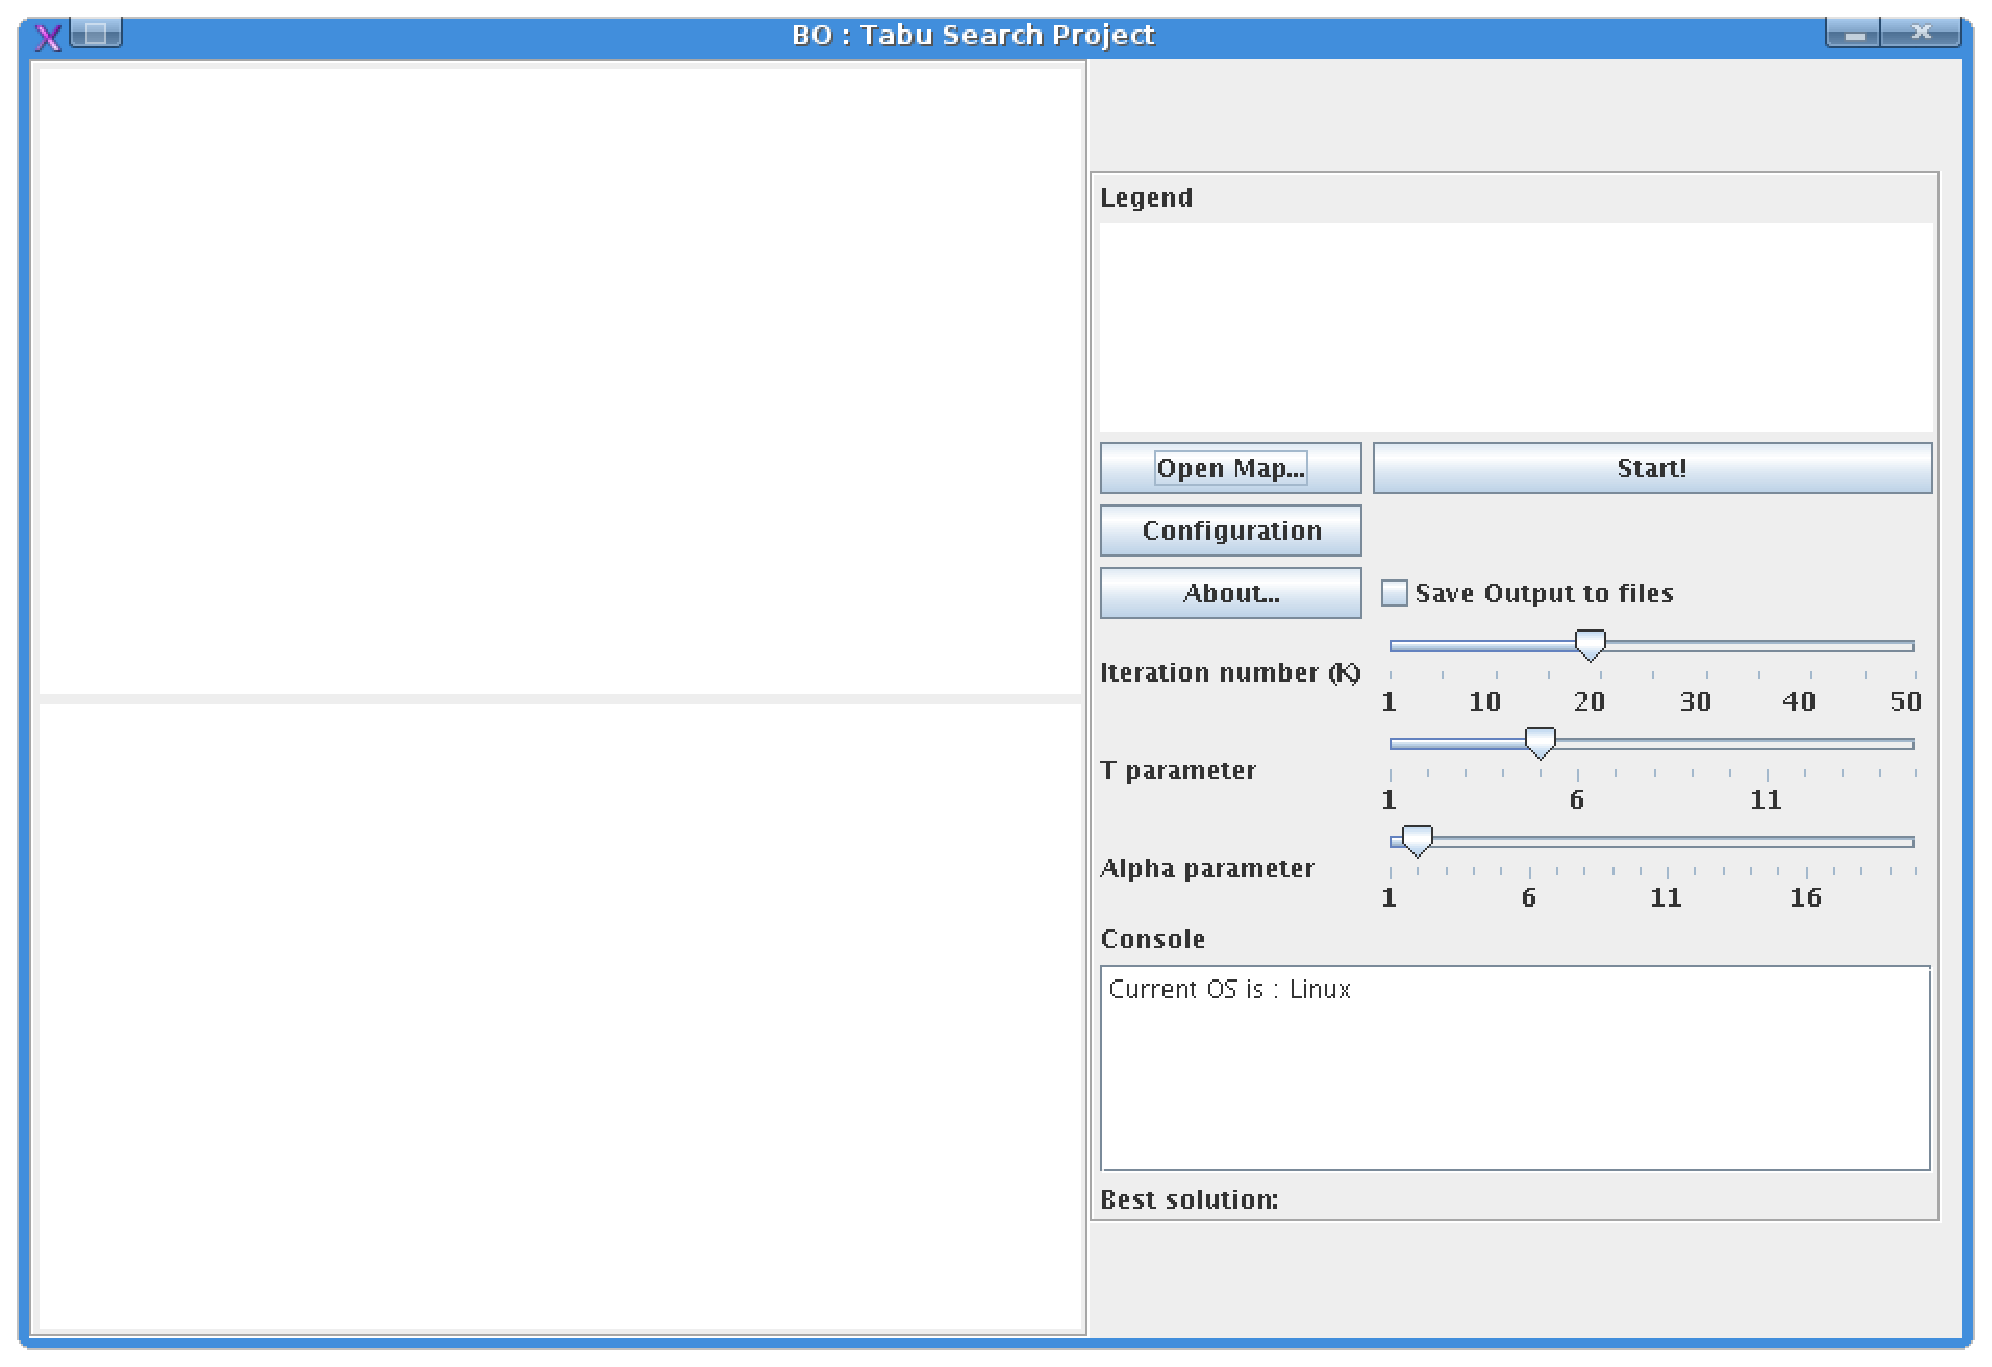
\includegraphics[width=0.75\textwidth]{./img/mainWnd.eps}
  \caption{G��wne okno programu}
  \label{fig:mainWnd}
\end{figure}
% 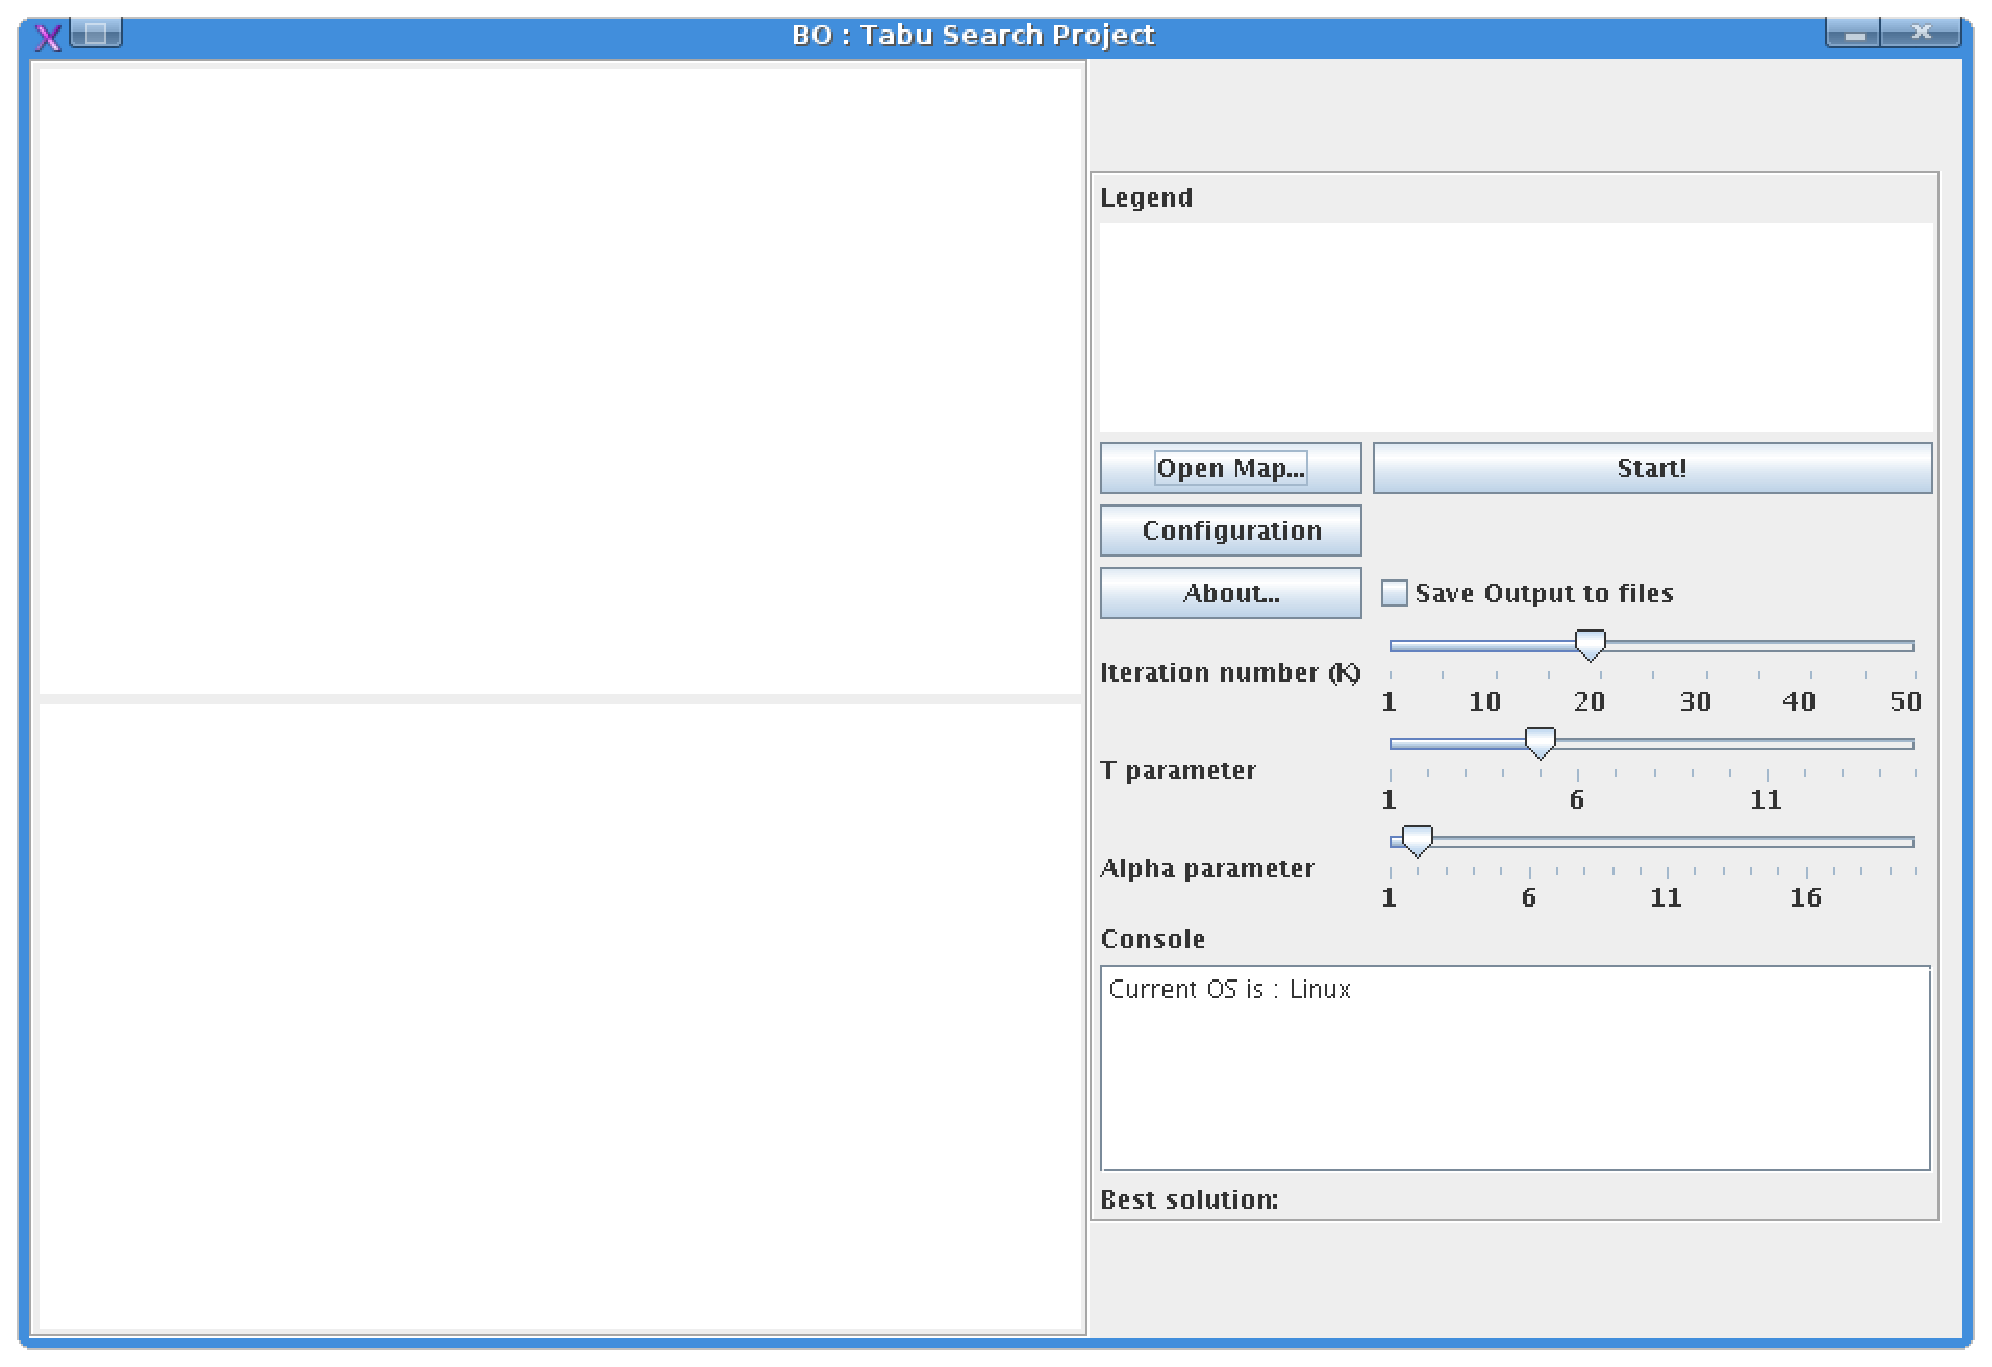
\includegraphics[width=1.0\textwidth]{./img/mainWnd.eps}\\[1cm]
Interfejs sk�ada sie z kilku podstawowych cz�ci: po lewej znajduj� si� obszary na kt�rych jest rysowane mapa i wykres funkcji celu. Po prawej znajduje si� legenda opisuj�ca map� ( przypisuje kolory do oznacze� budynk�w ) oraz przyciski steruj�ce dzia�aniem programu: \\
\begin{itemize}
  \item "Open Map..." - klikni�cie tego przycisku powoduje otwarcie okienka wyboru pliku zawieraj�cego map�. Za�adowanie pliku mapy jest niezb�dne do rozpocz�cia oblicze�. 

  \item "Configuration"- otwiera okno konfiguracji parametr�w (zyski z poszczeg�lnych typ�w budynk�w oraz opis anten: koszt i zasi�g). Program posiada pewne domy�ne parametry, wi�c konfiguracja nie jest obligatoryjna. Dok�adniejszy opis znajduje si� w dalszej cz�ci tej sekcji.

  \item "About" - otwiera okno opisuj�ce autor�w tego projektu

  \item "Save Output to files" - zaznaczenie tego pola pozwala na wybranie katalogu do zapisywania danych wyj�ciowych. Program zapisuje wyj�cie jako cztery pliki: 3 pliki PNG , zawieraj�ce map� wykres funkcji celu oraz legedn�, oraz jeden plik tekstowy w kt�rym znajduj� si� parametry z jakimi zosta�y wykonane obliczenia.

  \item "Start" przycisk kt�ry uruchamia obliczenia, lub je zatrzymuje je�eli zosta�y ju� rozpocz�te.
\end{itemize}

Ponadto na oknie g��wnym znajduj� si� r�wnie� suwaki do zmiany parametr�w: K, T, Aplha kt�re zosta�y opisane w poprzednich paragrafach.
\\
Na dole okna znajduje si� konsola na kt�r� s� wypisywane najwa�niejsze informacje o stanie dzia�ania programu. W niej pojawiaj� si� r�wnie� ostrze�enia o b��dach. Poni�ej konsoli znajduje si� etykieta na kt�rej wy�wietla si� informacja o najlepszym znalezionym rozwi�zaniu. \\
\subsubsection{Konfiguracja}
Okno konfiguracji znajduje si� na obrazie \ref{fig:confProfit}.
\begin{figure}
  \centering
  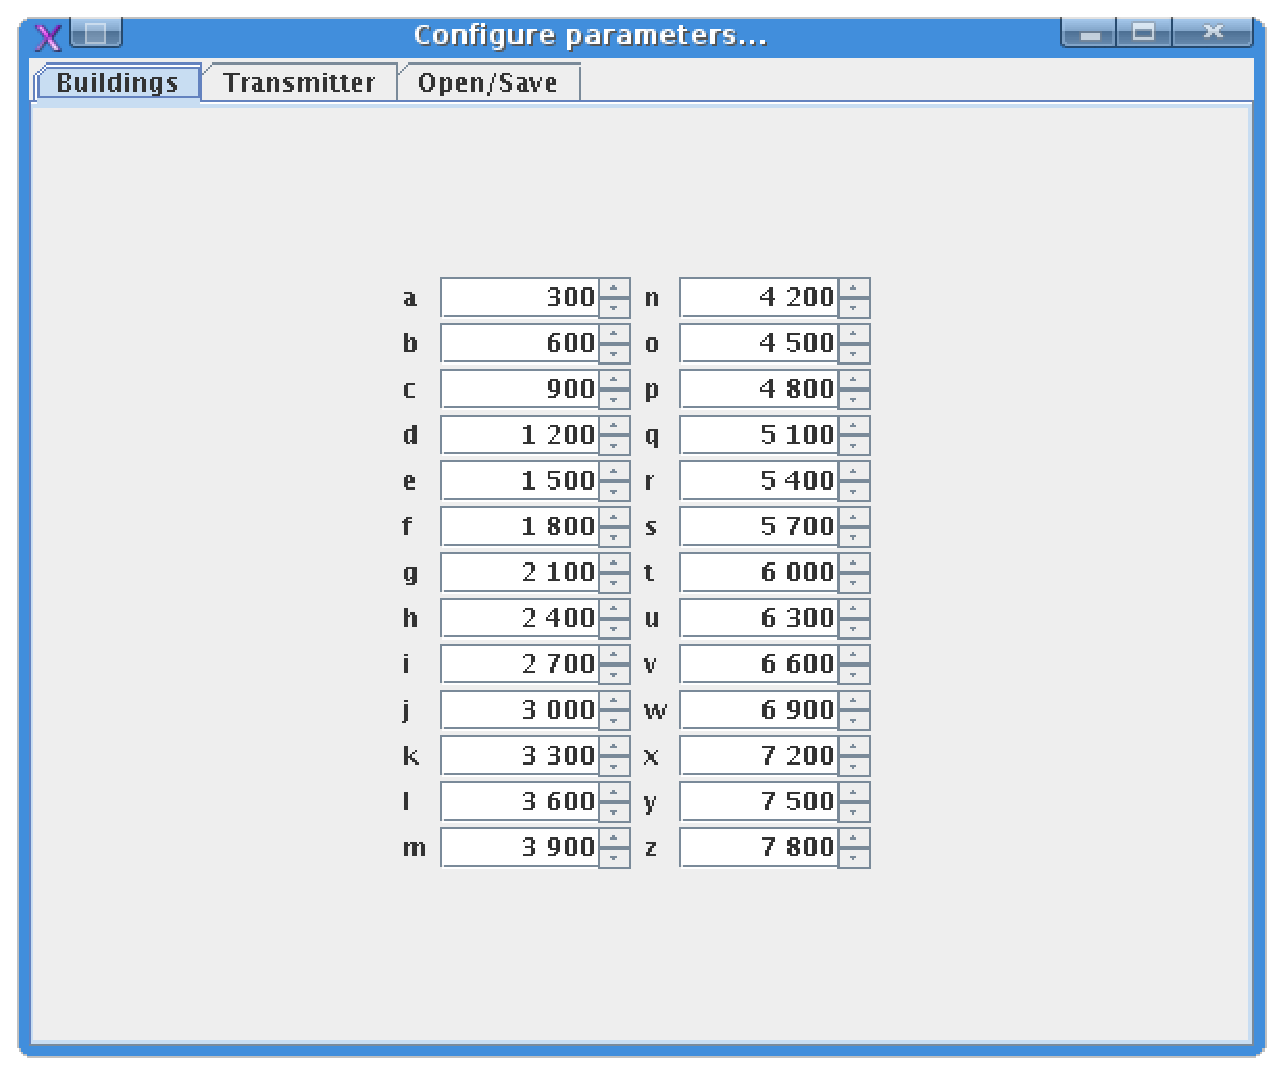
\includegraphics[width=0.75\textwidth]{./img/confWndProfit.eps}
  \caption{Okno konfiguracji: Edycja budynk�w}
  \label{fig:confProfit}
\end{figure}
% 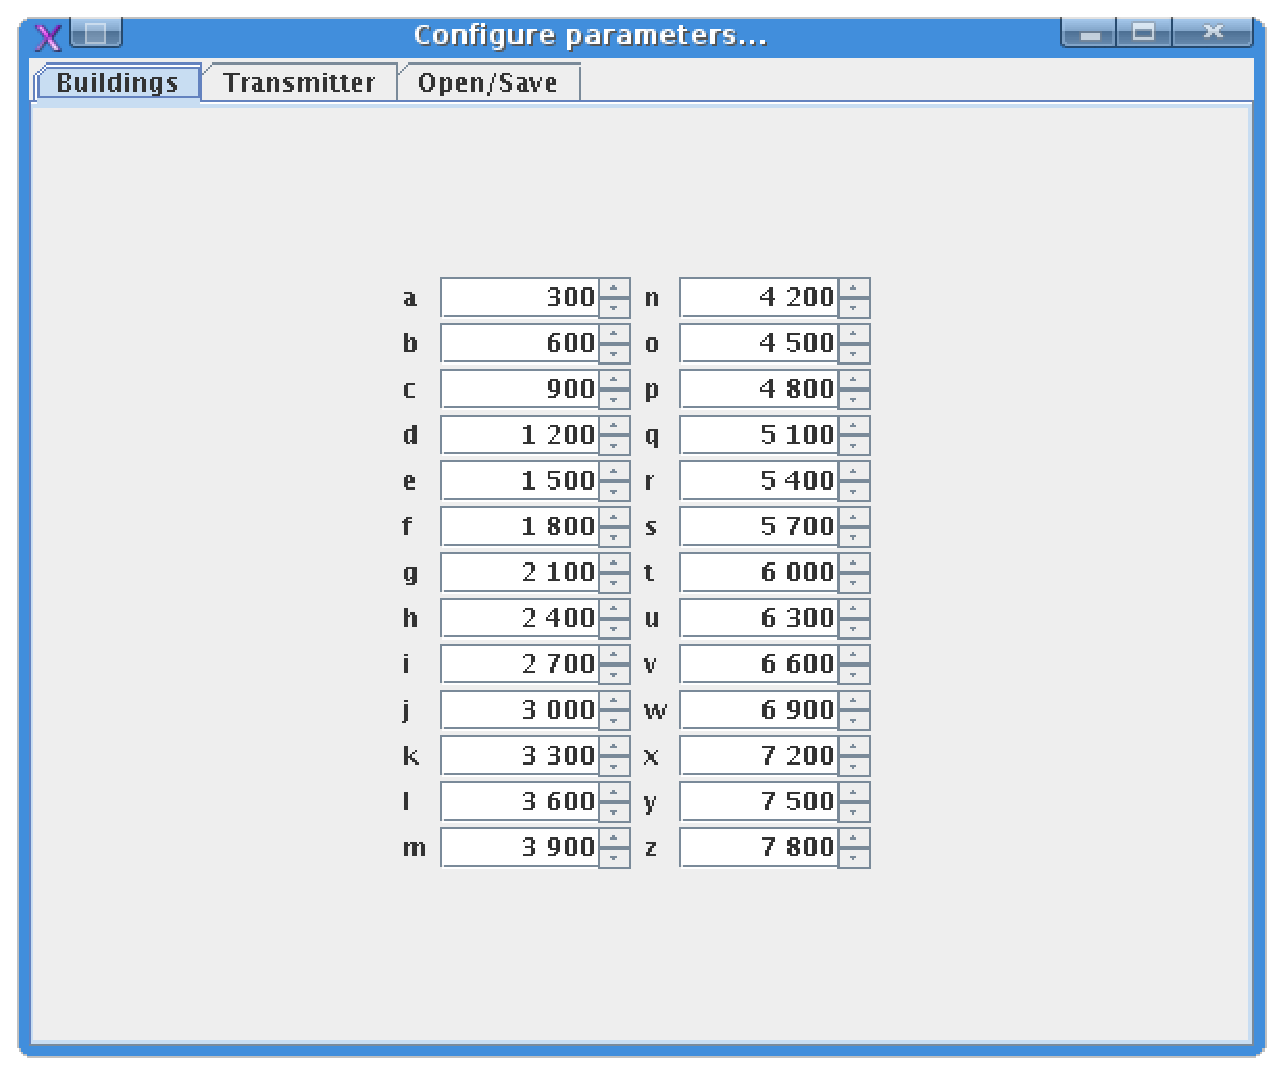
\includegraphics[width=1.0\textwidth]{./img/confWndProfit.eps}\\[1cm]
Tutaj pokazana jest konfiguracja zysk�w z obj�cia danego budynku zasi�giem. W naszym projekcie rozr�niamy budynki oznaczaj�c je literami alfabetu 'a' - 'z' (bez polskich liter). Ka�demu rodzajowi budynku mo�na przyporz�dkowa� dowolny nieujemny zysk. Przek�ada si� to na wygl�d mapy i oczywi�cie rezultat oblicze�.\\
Kolejn� zak�adk� jest konfiguracja anten pokazana na obrazie \ref{fig:confTrans}
\begin{figure}
  \centering
  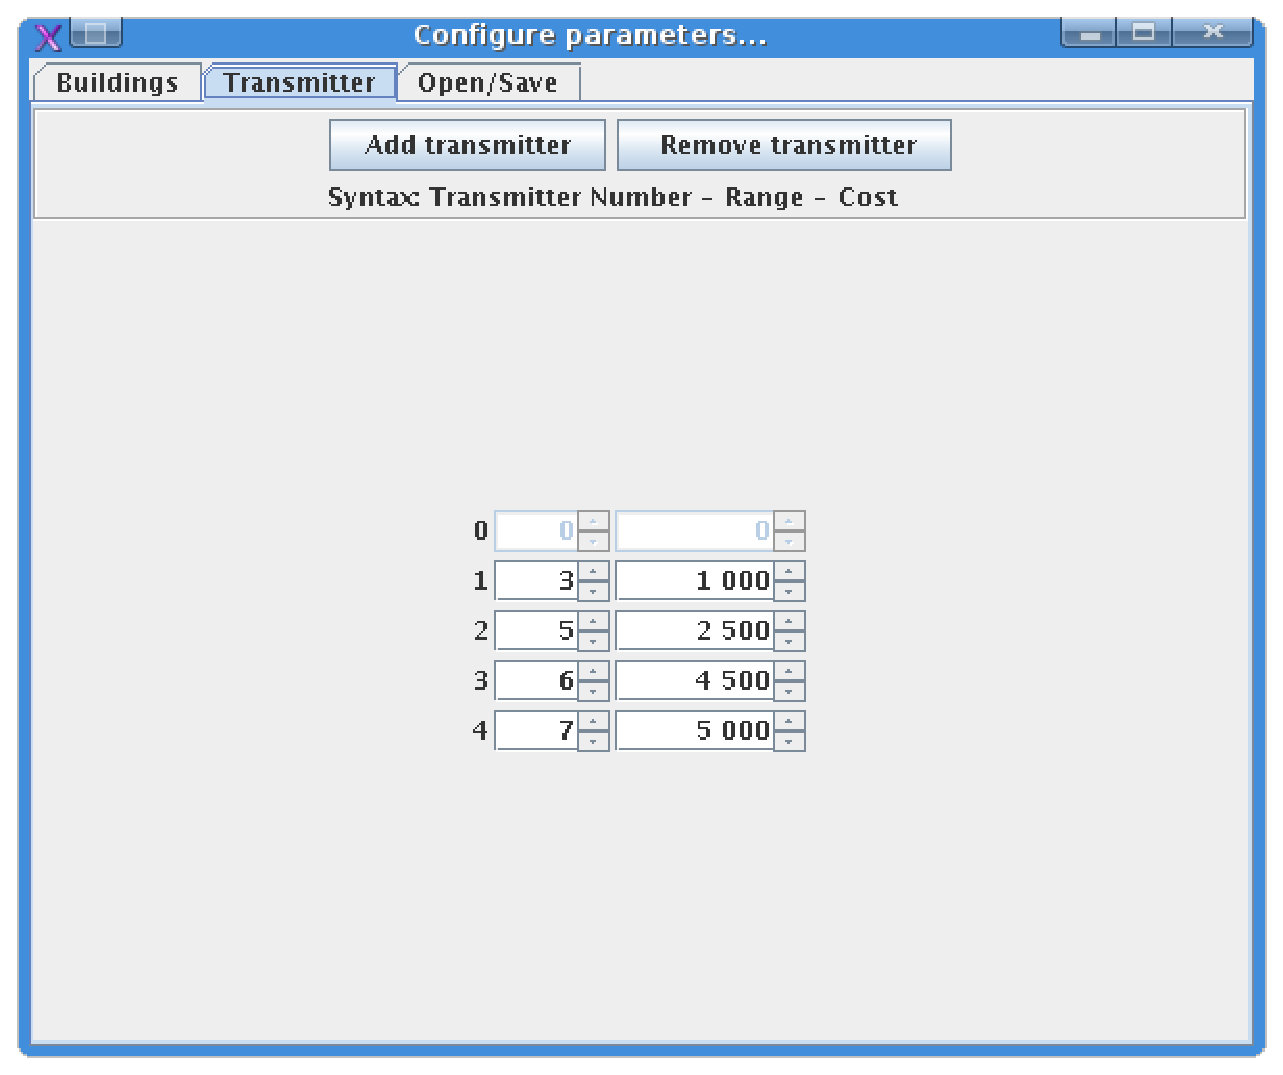
\includegraphics[width=0.75\textwidth]{./img/confWndTransEdit.eps}
  \caption{Okno konfiguracji: Anteny}
  \label{fig:confTrans}
\end{figure}
% 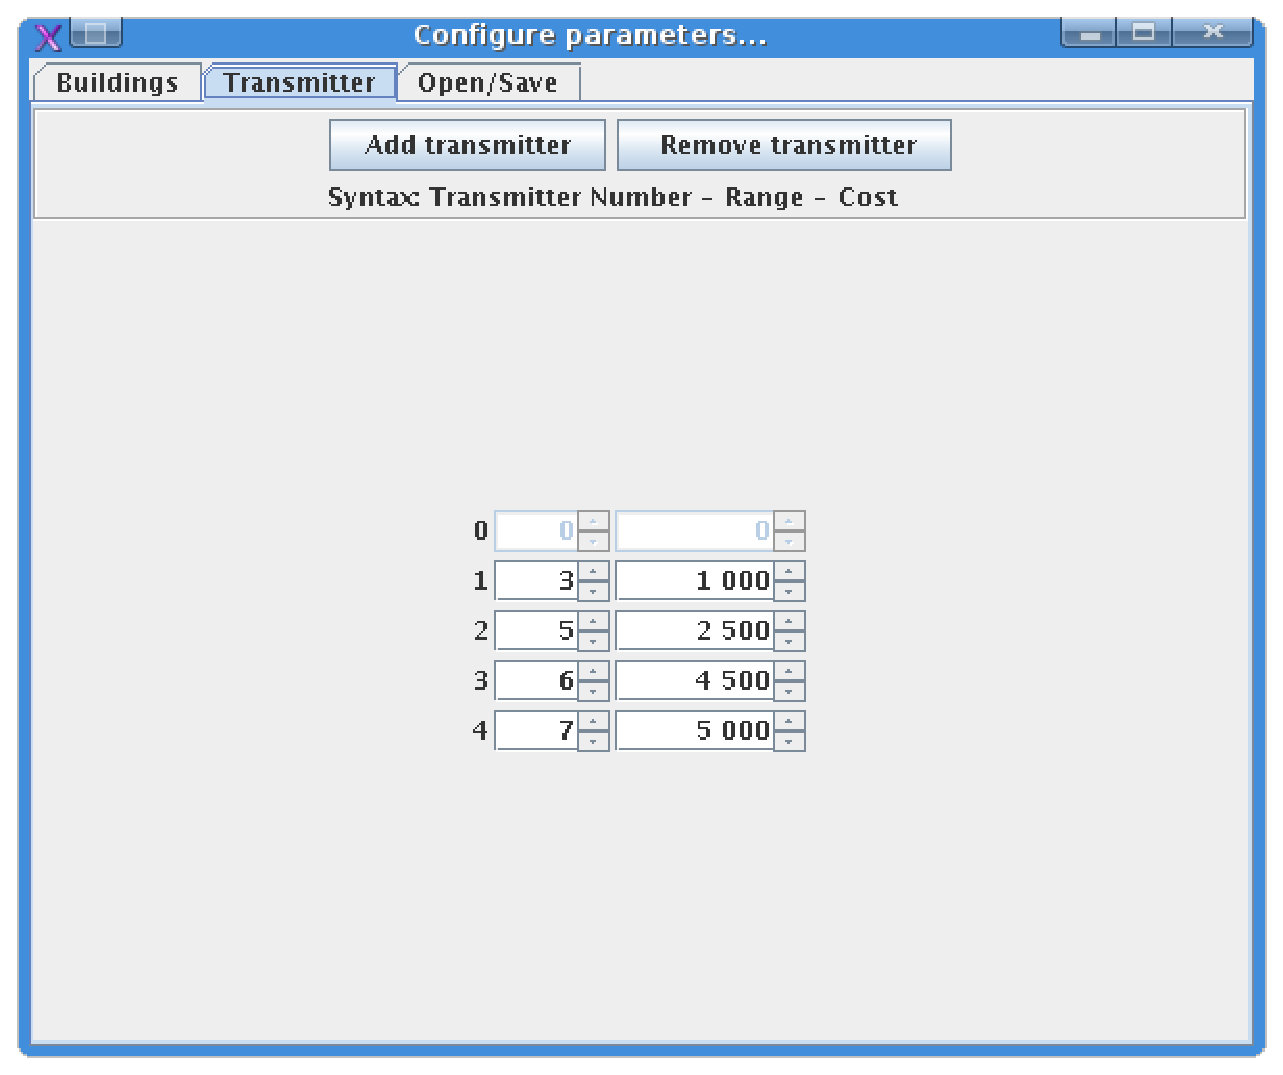
\includegraphics[width=1.0\textwidth]{./img/confWndTransEdit.eps}\\[1cm]
Klikni�cie na przycisk "Add transmitter" powoduje dodanie nowej anteny do listy. Ka�d� anten�, opr�cz zerowej, mo�na edytowa� tzn. ustala� jej zasi�g oraz koszt postawienia. Pierwsze pole odpowiada za zasi�g, a drugie za koszt.\\ Klikaj�c na przycisk "Remove transmitter" usuwamy anten� z listy. Nie mo�na usun�� tylko anteny "zerowej".
Ostatnia zak�adka s�u�y do zatwierdzenia konfiguracji, anulowania zmian, zapisania jej do pliku lub otwarcia istniej�cej zapisanej konfiguracji, zrzut ekranu z t� zak�adk� znajduje si� na obrazie \ref{fig:confFiles}\\
\begin{figure}
  \centering
  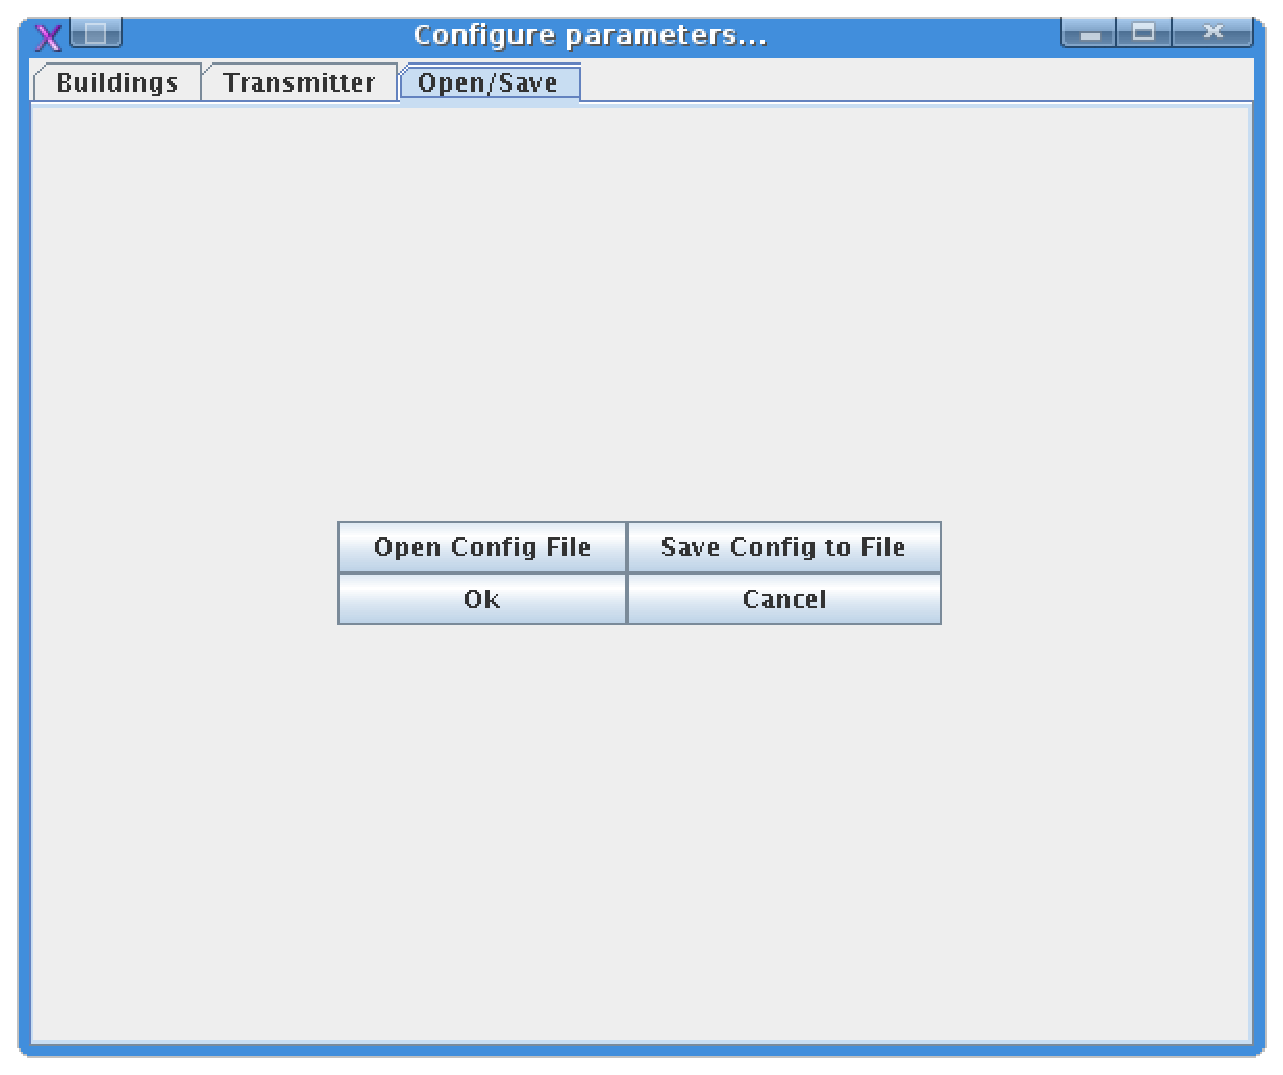
\includegraphics[width=0.75\textwidth]{./img/confWndFiles.eps}
  \caption{Okno konfiguracji: Otwieranie i zapisywanie konfiguracji}
  \label{fig:confFiles}
\end{figure}
% 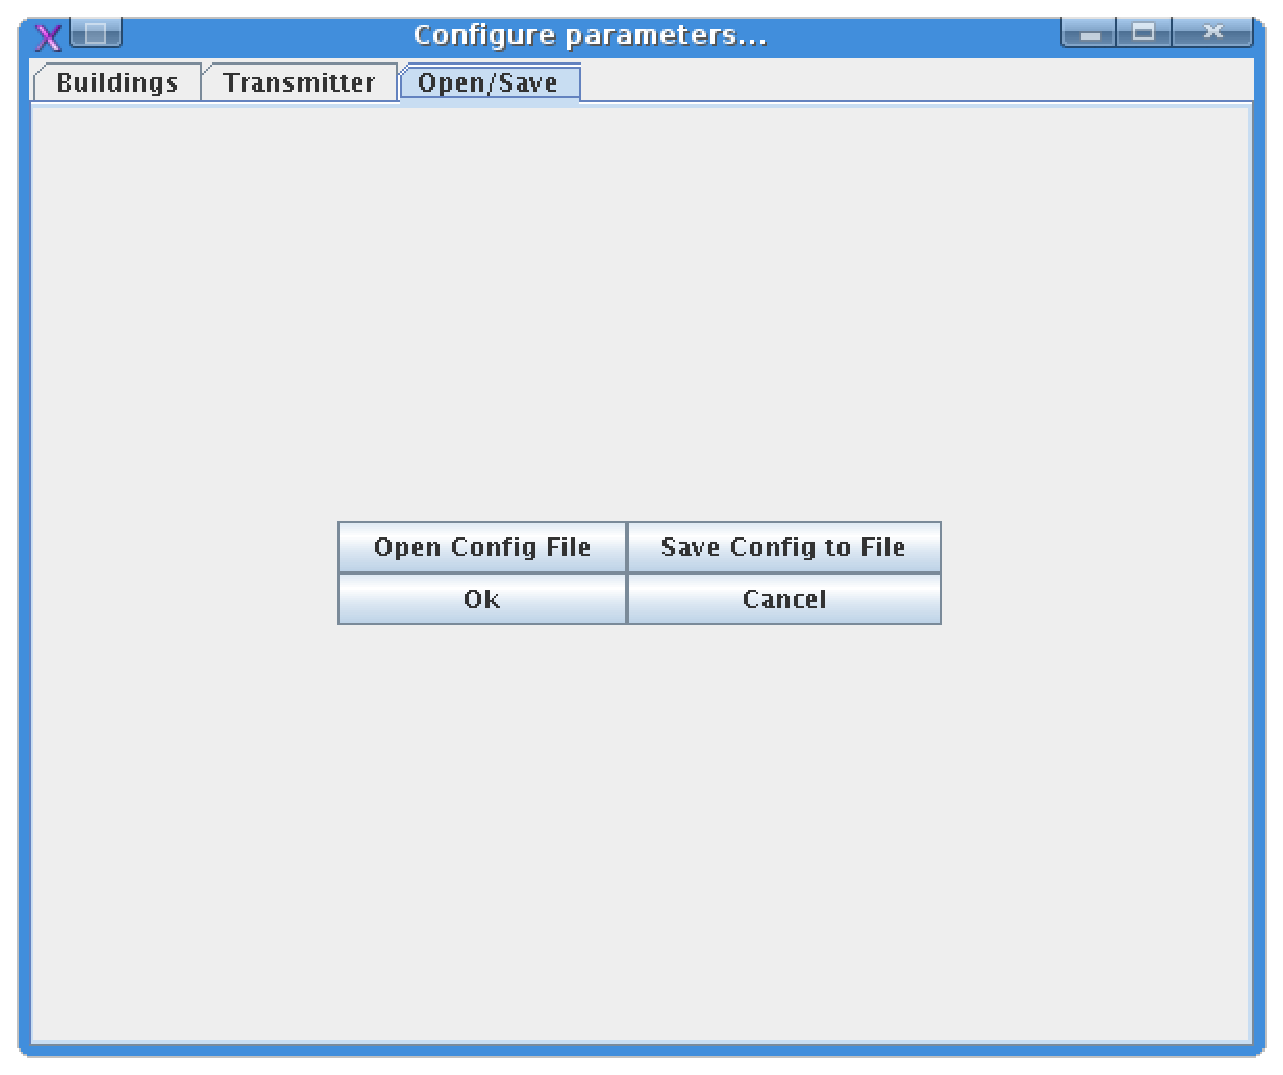
\includegraphics[width=1.0\textwidth]{./img/confWndFiles.eps}\\[1cm]
\subsubsection{Dzia�anie}
Pierwszym krokiem jest wczytanie mapy. Jest ona nast�pnie parsowana i na tej podstawie jest rysowana graficzna jej reprezentacja. Uruchomienie procesu obliczeniowego odbywa si� przez wci�ni�cie przycisku "Start". Powoduje to utworzenie nowego w�tku, w kt�rym jest wywo�ywany program "processor". Po jego zako�czeniu GUI analizuje jego wyj�cie i przetwarza je na obraz rozwi�zania (tzn zaznaczenie wybranych nadajnik�w oraz obrysowanie ich zasiegu) oraz rysuje wykres funkcji celu dla kolejnych iteracji. \\ Je�eli nie zosta�a zmieniona domy�nla konfiguracja to program korzysta z niej i nie przekazuje �adnej informacji jej dotycz�cej do "processora". W przeciwnym przypadku u�ytkownik musi najpierw zapisa� konfiguracj� do pliku, aby mog�a zosta� przekazana do procesu obliczeniowego.\\
Je�eli u�ytkownik zaznaczy� opcj� zapisu wyj�cia do pliku to zostan� wygenerowane pliki we wskazanym folderze. Generowane s� nast�puj�ce pliki o sk�adni:
\begin{itemize}
  \item \textit{<input\_file>\_graph.png} - obraz funkcji celu;
  \item \textit{<input\_file>\_map.png} - wizualizacja mapy;
  \item \textit{<input\_file>\_legend.png} - plik z obrazem legendy;
  \item \textit{<input\_file>\_config.txt} - plik tekstowy z informacj� o konfiguracji z jak� dane wej�ciowe by�y przetwarzane;
\end{itemize}
<input\_file> to nazwa pliku wej�ciowego (mapy).\\

\section{Testowanie}
Aby przekona� si� o poprawno�ci wykonanego programu wykonali�my seri� test�w na r�nych mapach pr�bnych. Chcieli�my si� r�wnie� przekona� o wydajno�ci zaimplementowanego algorytmu. Poniewa� zosta� on zaprogramowany w C++ bez zb�dnego "baga�u" interfejsu spodziewali�my si� do�� du�ej wydajno�ci. Na kolejnych obrazkach i tabelkach znajduj� si� rozwi�zania znalezione przez program wraz z podanym zyskiem i czasem oblicze� (ten mo�e by� nieco wi�kszy ni� realny czas wykonania samego programu przetwarzaj�cego, gdy� jest mierzony z poziomu GUI co oznacza pewien narzut zwi�zany odczytem wyj�cia procesu obliczeniowego).

\begin{figure}[!h]
  \centering
  \subfigure[Mapka za na�o�onym rozwi�zaniem]{\label{fig:map01_out}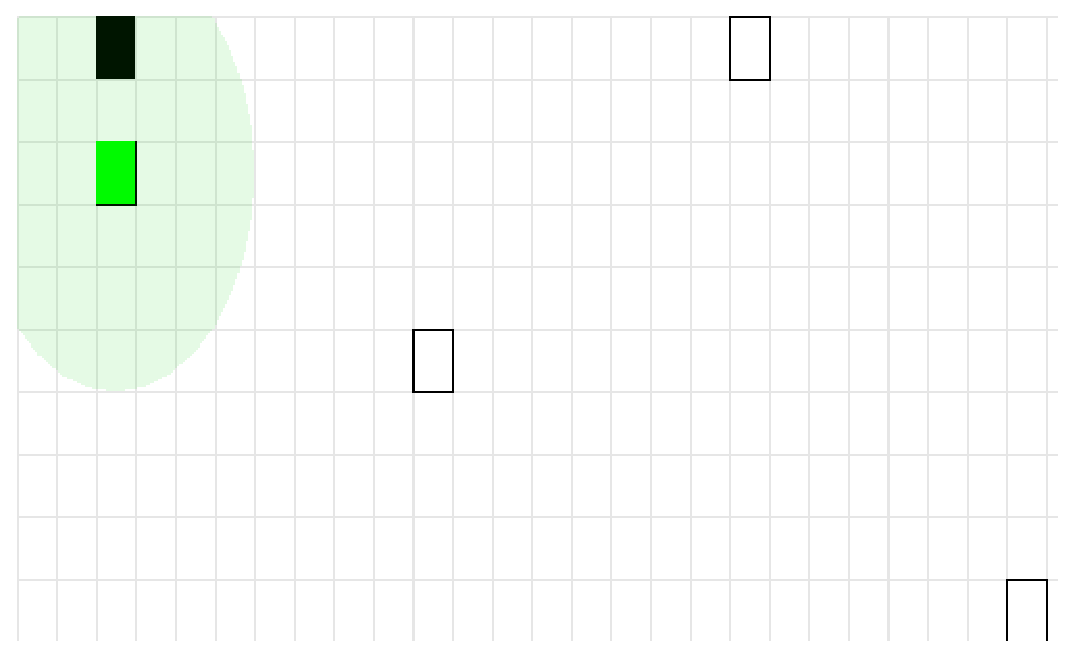
\includegraphics[width=0.45\textwidth]{./img/output/map01_map.eps}}
  \subfigure[Wykres funkcji celu]{\label{fig:map01_func}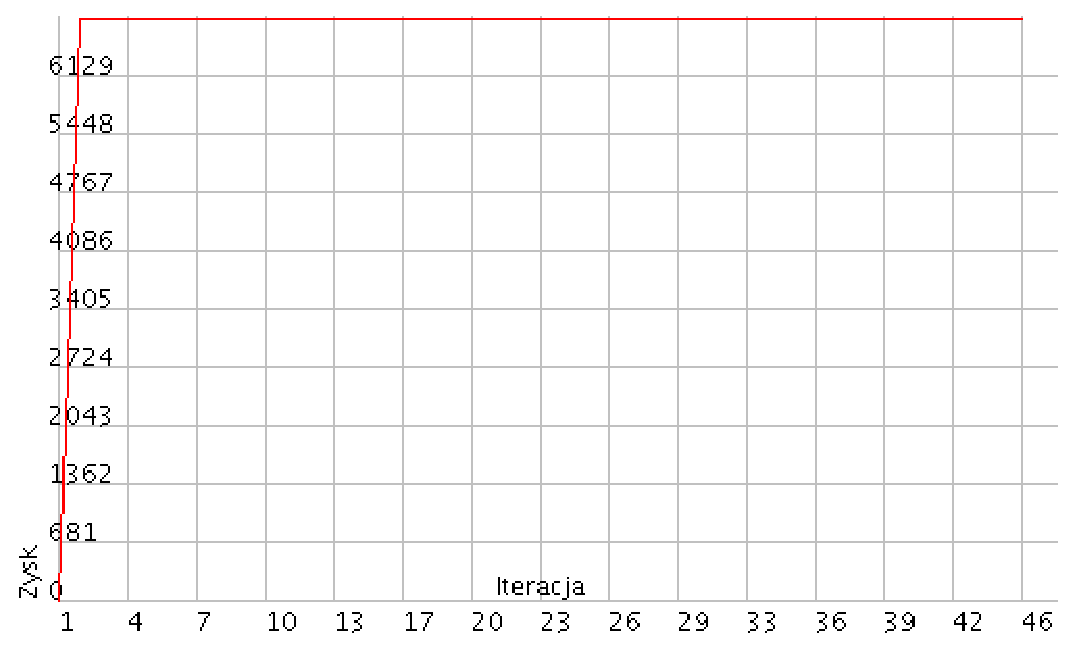
\includegraphics[width=0.45\textwidth]{./img/output/map01_graph.eps}}
  \caption{Mapa map01 : rozwi�zanie oraz wykres funkcji celu}
  \label{fig:map01}
\end{figure}

\begin{figure}
  \centering
  \subfigure[Mapka za na�o�onym rozwi�zaniem]{\label{fig:map02_out}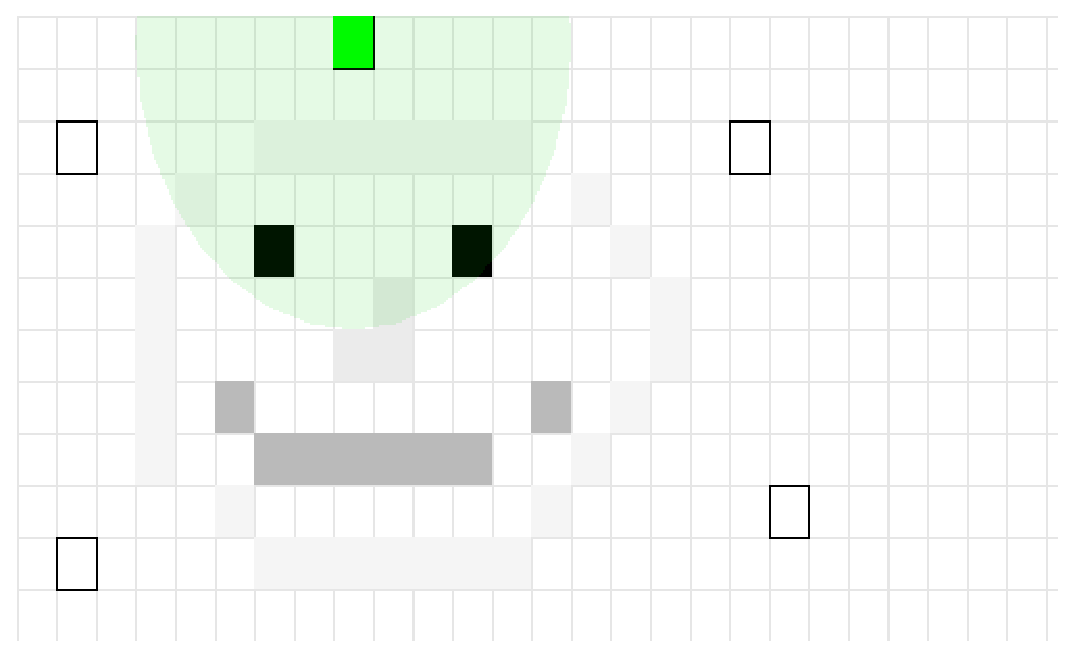
\includegraphics[width=0.45\textwidth]{./img/output/map02_map.eps}}
  \subfigure[Wykres funkcji celu]{\label{fig:map02_func}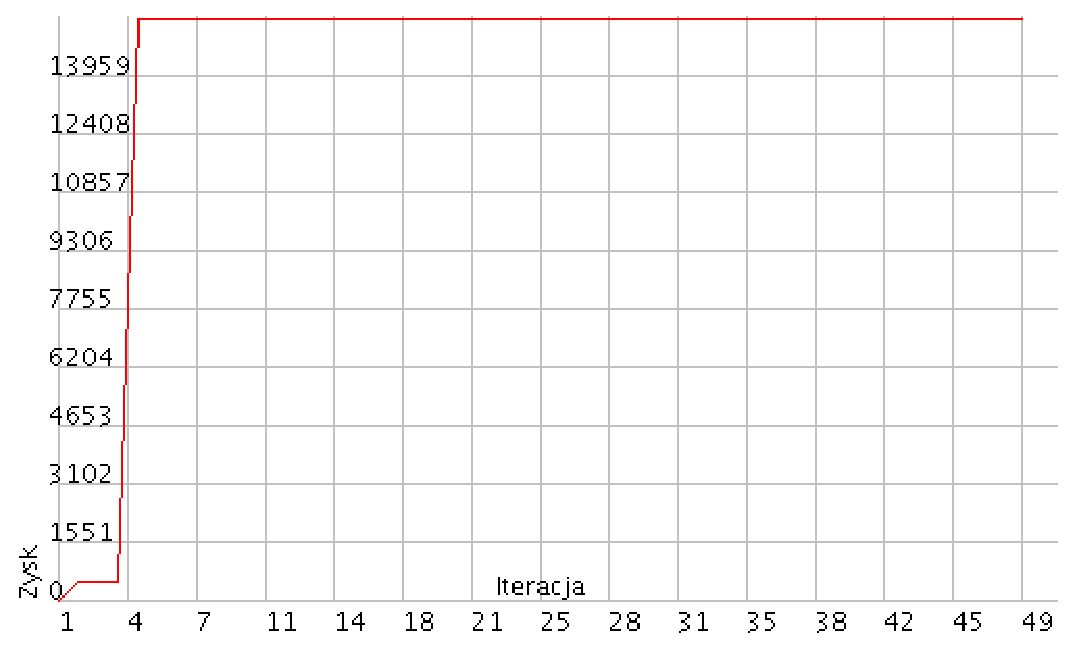
\includegraphics[width=0.45\textwidth]{./img/output/map02_graph.eps}}
  \caption{Mapa map02 : rozwi�zanie oraz wykres funkcji celu}
  \label{fig:map02}
\end{figure}

\begin{figure}
  \centering
  \subfigure[Mapka za na�o�onym rozwi�zaniem]{\label{fig:map03_out}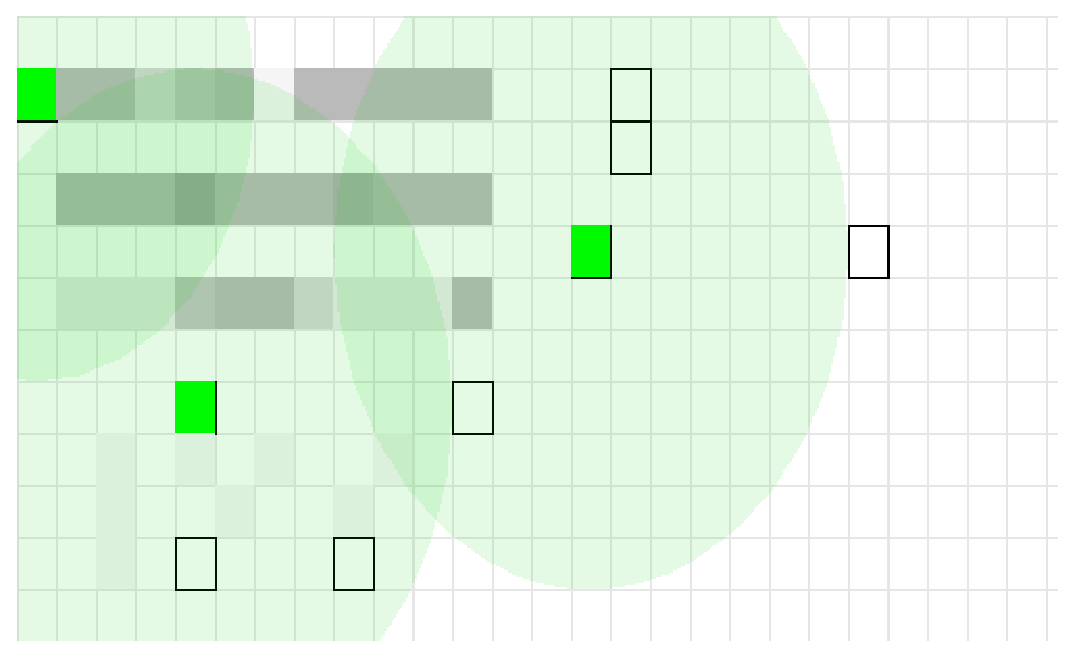
\includegraphics[width=0.45\textwidth]{./img/output/map03_map.eps}}
  \subfigure[Wykres funkcji celu]{\label{fig:map03_func}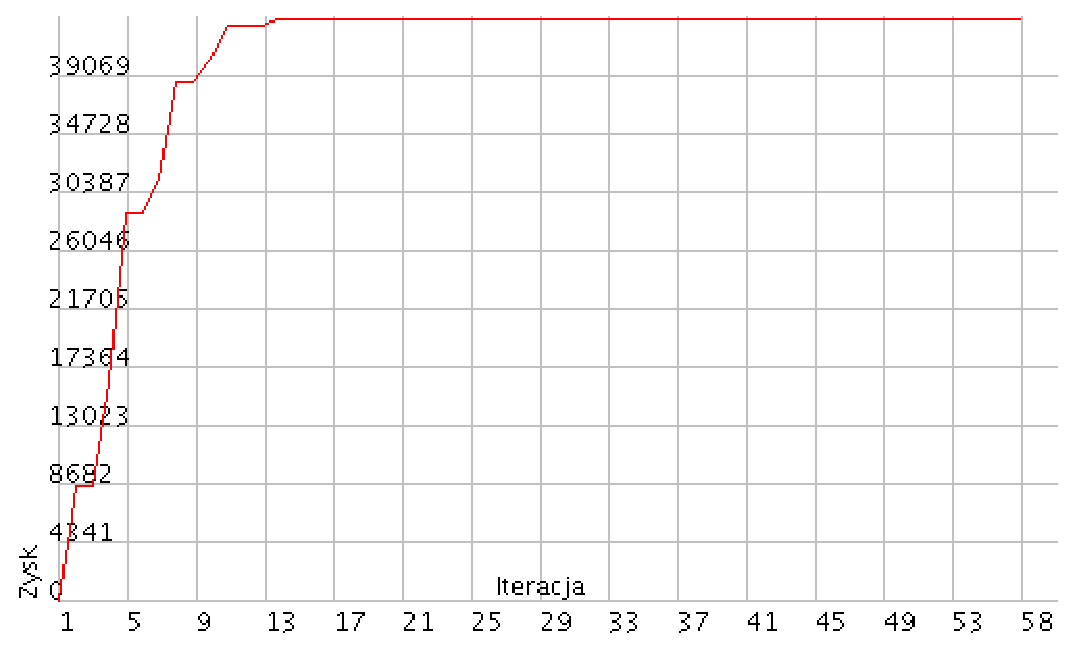
\includegraphics[width=0.45\textwidth]{./img/output/map03_graph.eps}}
  \caption{Mapa map03 : rozwi�zanie oraz wykres funkcji celu}
  \label{fig:map03}
\end{figure}

\begin{figure}
  \centering
  \subfigure[Mapka za na�o�onym rozwi�zaniem]{\label{fig:map04_out}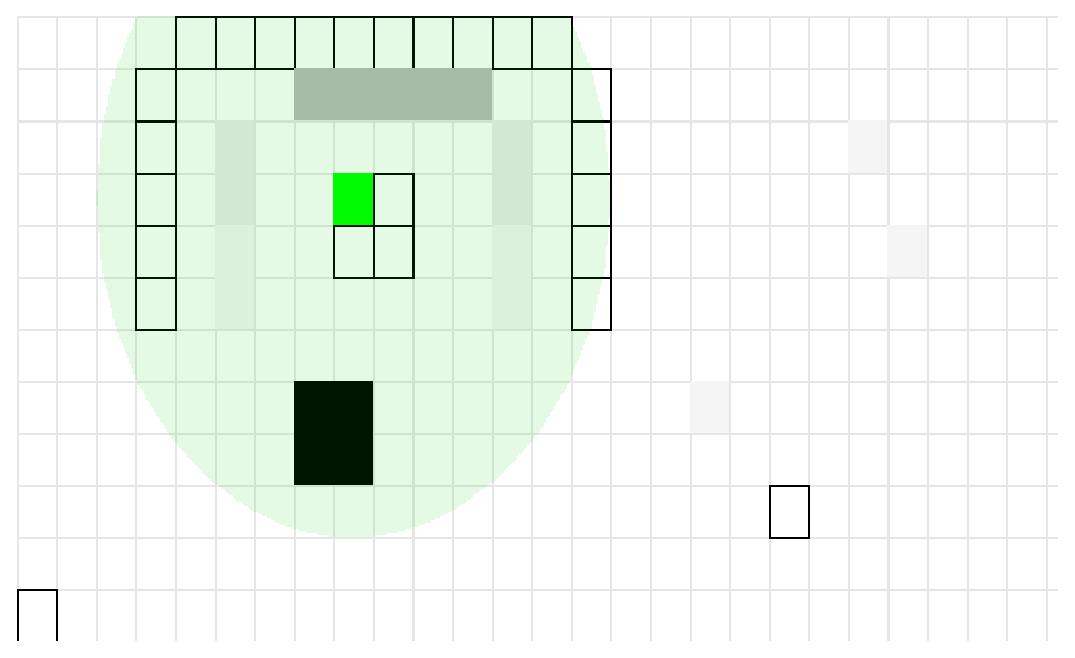
\includegraphics[width=0.45\textwidth]{./img/output/map04_map.eps}}
  \subfigure[Wykres funkcji celu]{\label{fig:map04_func}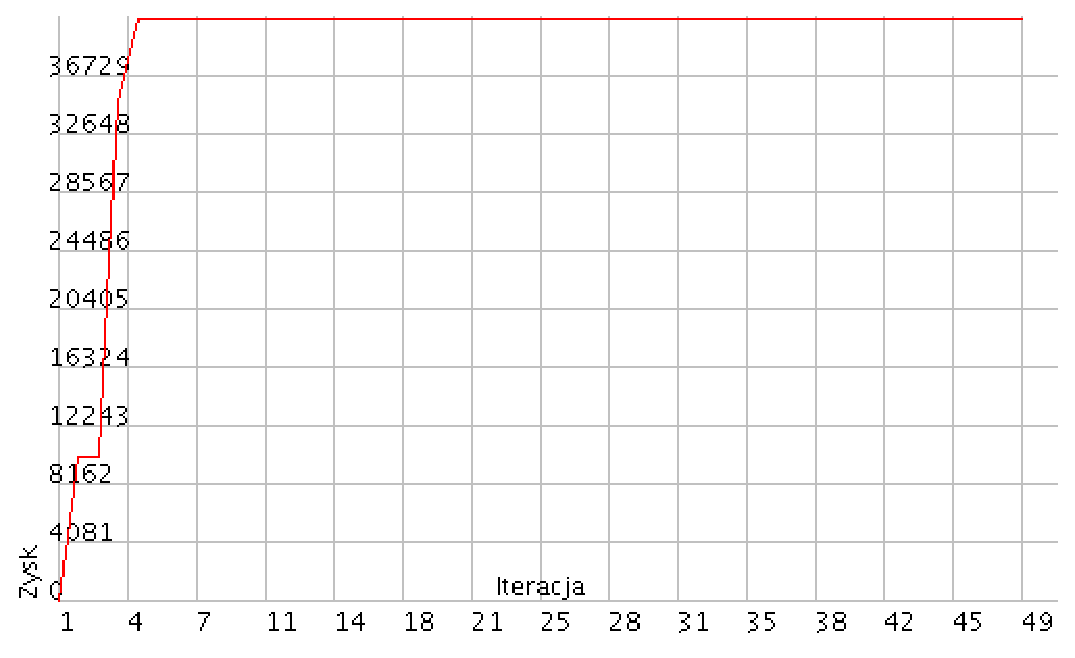
\includegraphics[width=0.45\textwidth]{./img/output/map04_graph.eps}}
  \caption{Mapa map04 : rozwi�zanie oraz wykres funkcji celu}
  \label{fig:map04}
\end{figure}

\begin{figure}
  \centering
  \subfigure[Mapka za na�o�onym rozwi�zaniem]{\label{fig:map05_out}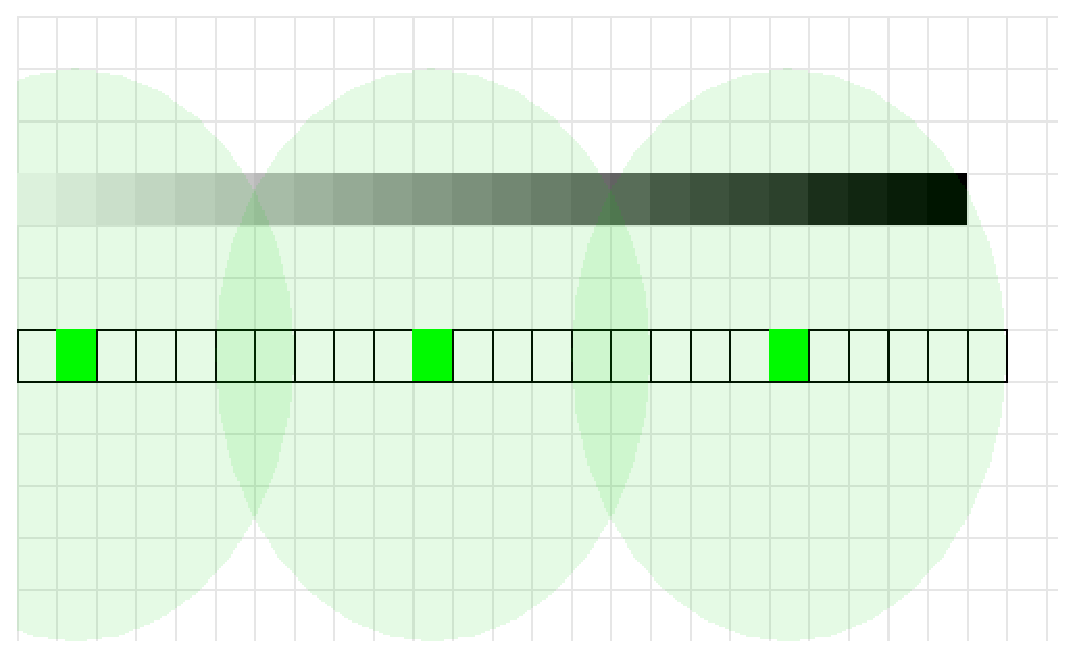
\includegraphics[width=0.45\textwidth]{./img/output/map05_map.eps}}
  \subfigure[Wykres funkcji celu]{\label{fig:map05_func}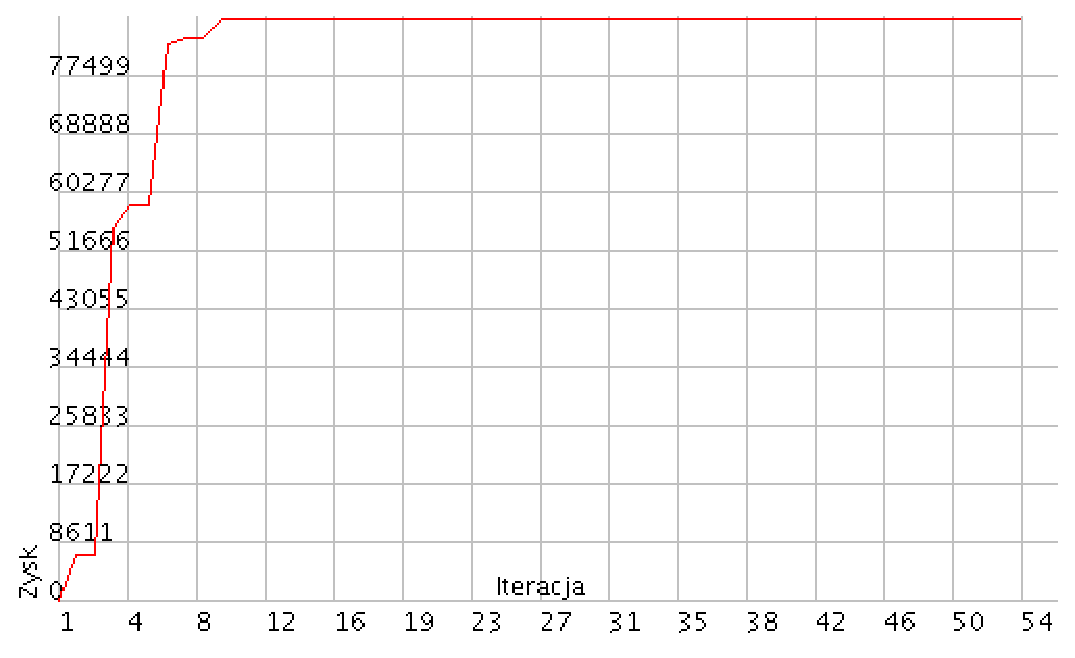
\includegraphics[width=0.45\textwidth]{./img/output/map05_graph.eps}}
  \caption{Mapa map05 : rozwi�zanie oraz wykres funkcji celu}
  \label{fig:map05}
\end{figure}

\begin{figure}
  \centering
  \subfigure[Mapka za na�o�onym rozwi�zaniem]{\label{fig:map06_out}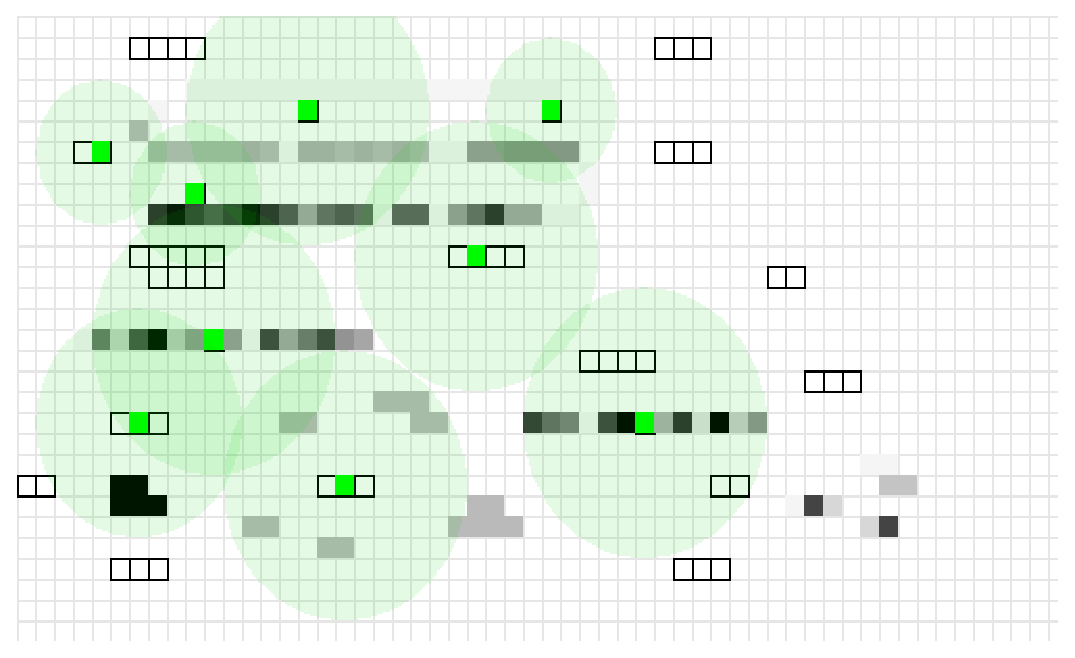
\includegraphics[width=0.45\textwidth]{./img/output/map06_map.eps}}
  \subfigure[Wykres funkcji celu]{\label{fig:map06_func}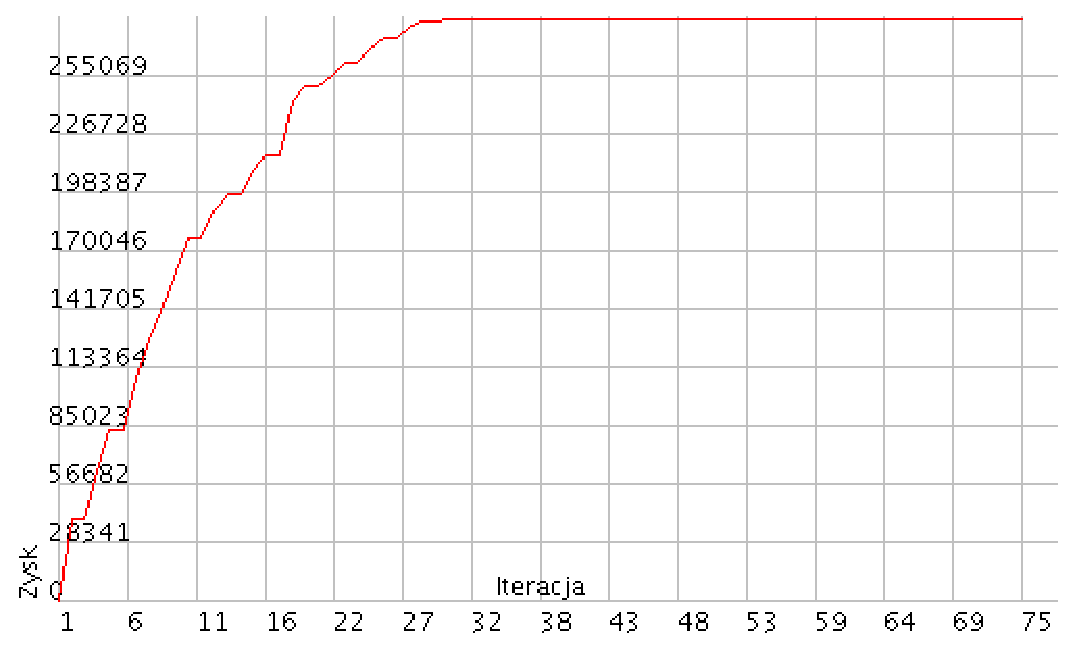
\includegraphics[width=0.45\textwidth]{./img/output/map06_graph.eps}}
  \caption{Mapa map06 : rozwi�zanie oraz wykres funkcji celu}
  \label{fig:map06}
\end{figure}

\begin{figure}
  \centering
  \subfigure[Mapka za na�o�onym rozwi�zaniem]{\label{fig:map07_out}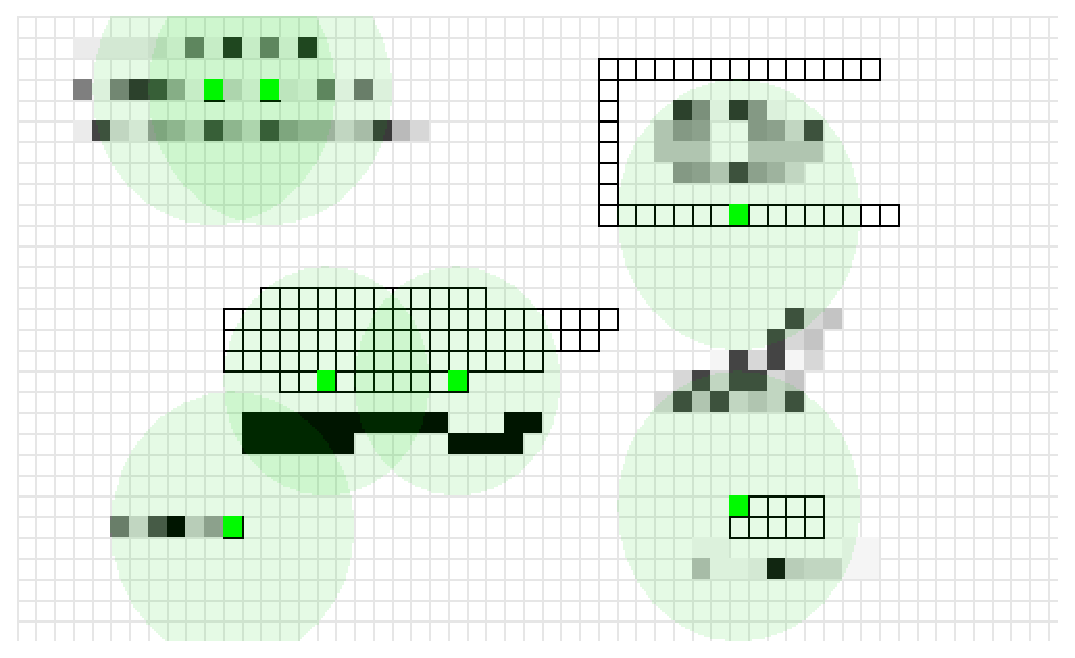
\includegraphics[width=0.45\textwidth]{./img/output/map07_map.eps}}
  \subfigure[Wykres funkcji celu]{\label{fig:map07_func}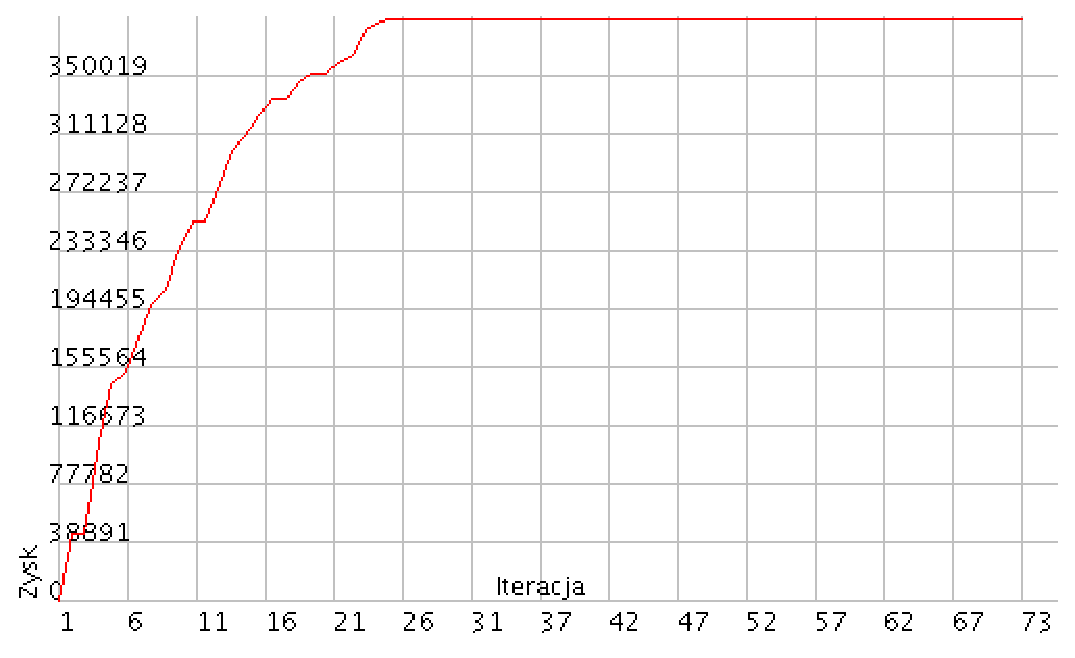
\includegraphics[width=0.45\textwidth]{./img/output/map07_graph.eps}}
  \caption{Mapa map07 : rozwi�zanie oraz wykres funkcji celu}
  \label{fig:map07}
\end{figure}

\begin{figure}
  \centering
  \subfigure[Mapka za na�o�onym rozwi�zaniem]{\label{fig:map08_out}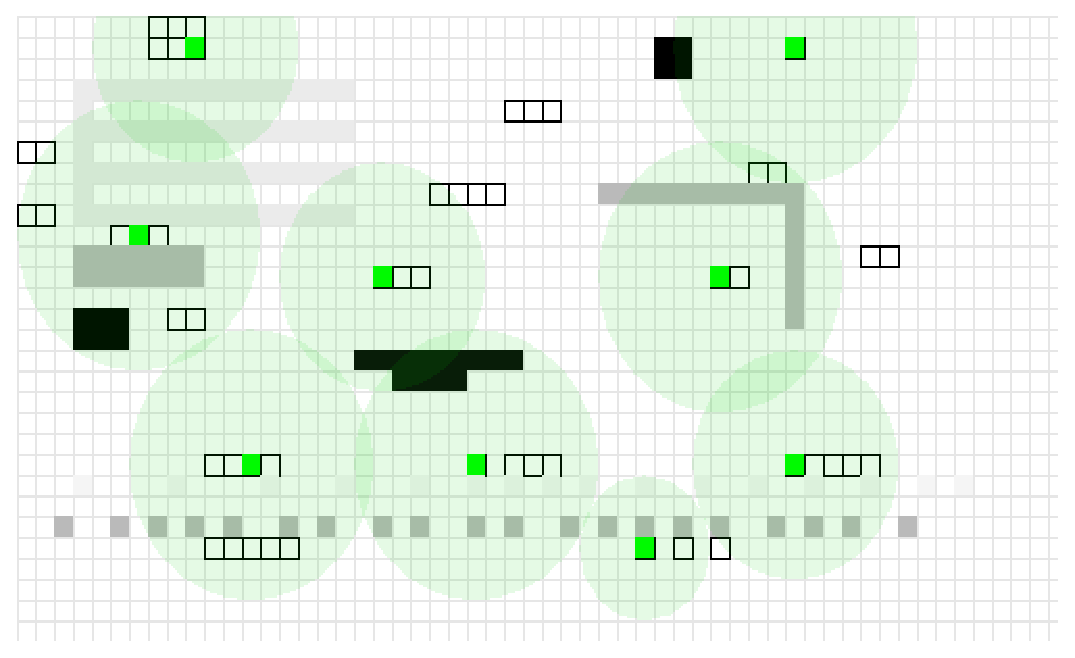
\includegraphics[width=0.45\textwidth]{./img/output/map08_map.eps}}
  \subfigure[Wykres funkcji celu]{\label{fig:map08_func}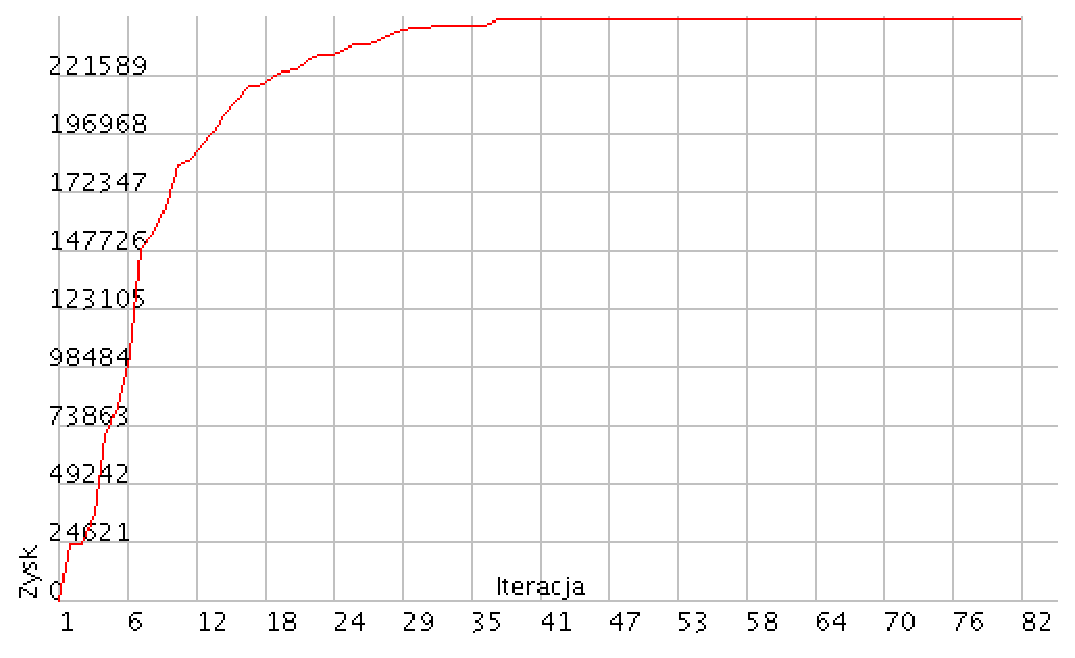
\includegraphics[width=0.45\textwidth]{./img/output/map08_graph.eps}}
  \caption{Mapa map08 : rozwi�zanie oraz wykres funkcji celu}
  \label{fig:map08}
\end{figure}

\begin{figure}
  \centering
  \subfigure[Mapka za na�o�onym rozwi�zaniem]{\label{fig:map09_out}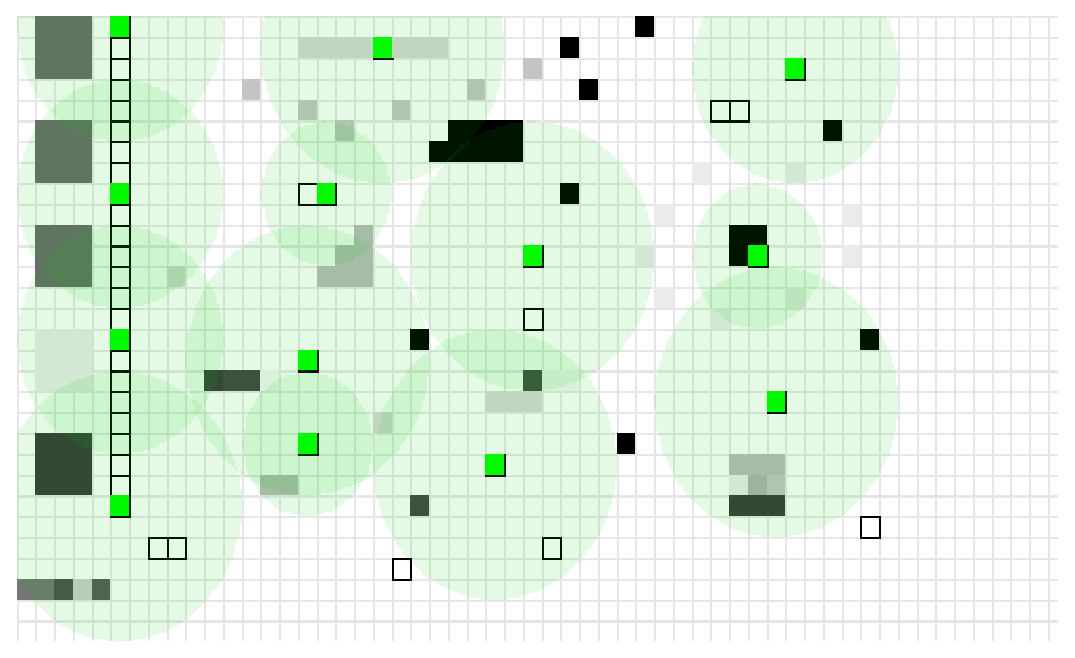
\includegraphics[width=0.45\textwidth]{./img/output/map09_map.eps}}
  \subfigure[Wykres funkcji celu]{\label{fig:map09_func}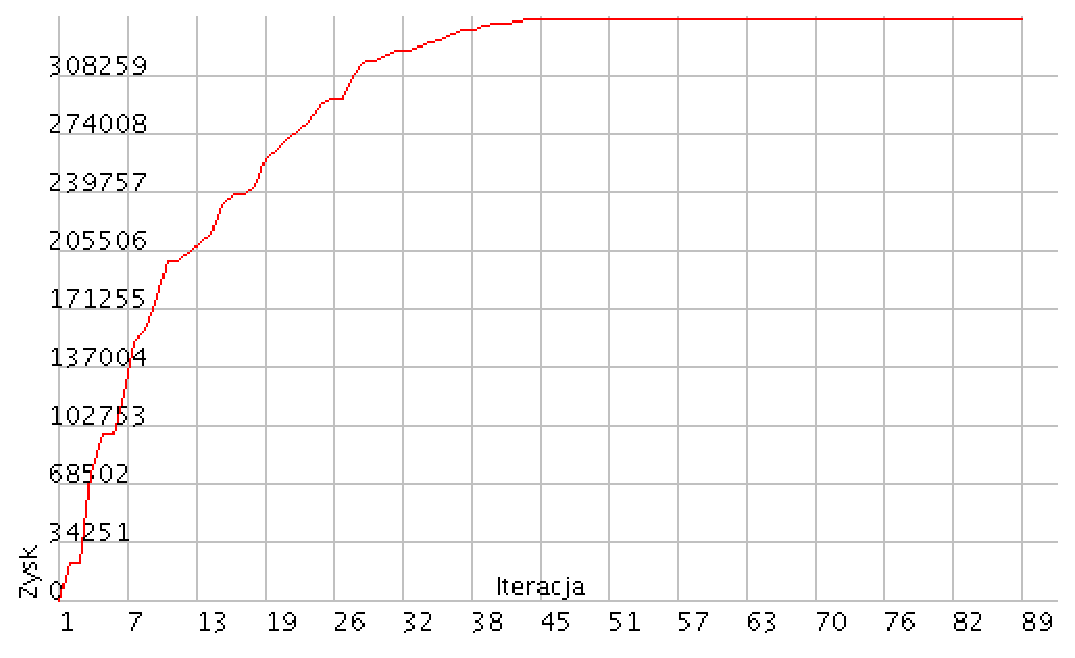
\includegraphics[width=0.45\textwidth]{./img/output/map09_graph.eps}}
  \caption{Mapa map09 : rozwi�zanie oraz wykres funkcji celu}
  \label{fig:map09}
\end{figure}

\begin{figure}
  \centering
  \subfigure[Mapka za na�o�onym rozwi�zaniem]{\label{fig:map10_out}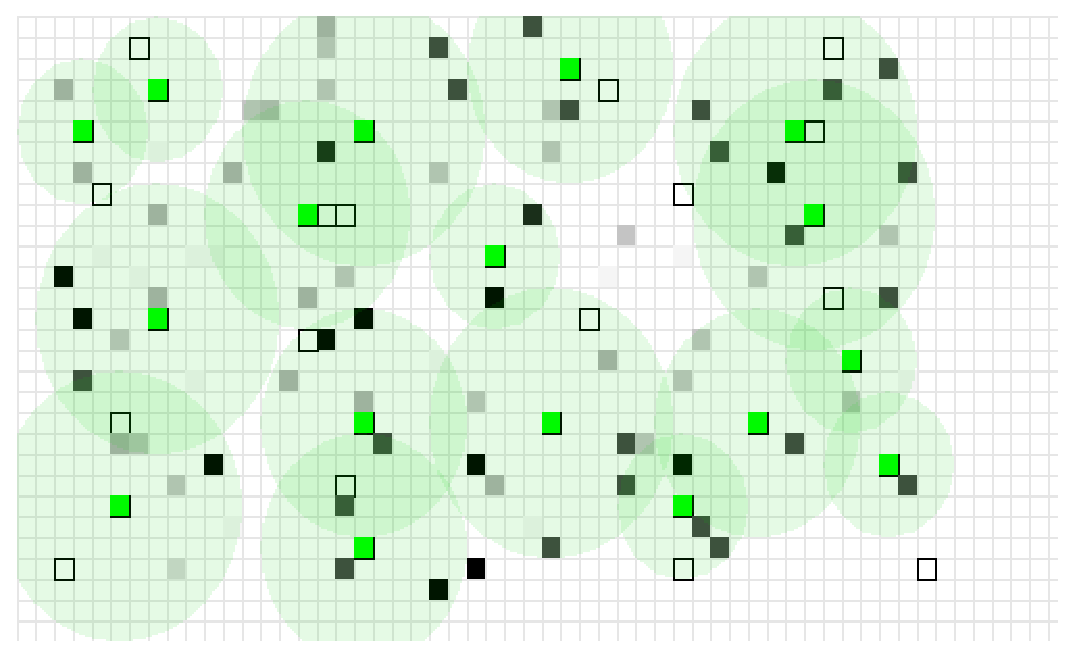
\includegraphics[width=0.45\textwidth]{./img/output/map10_map.eps}}
  \subfigure[Wykres funkcji celu]{\label{fig:map10_func}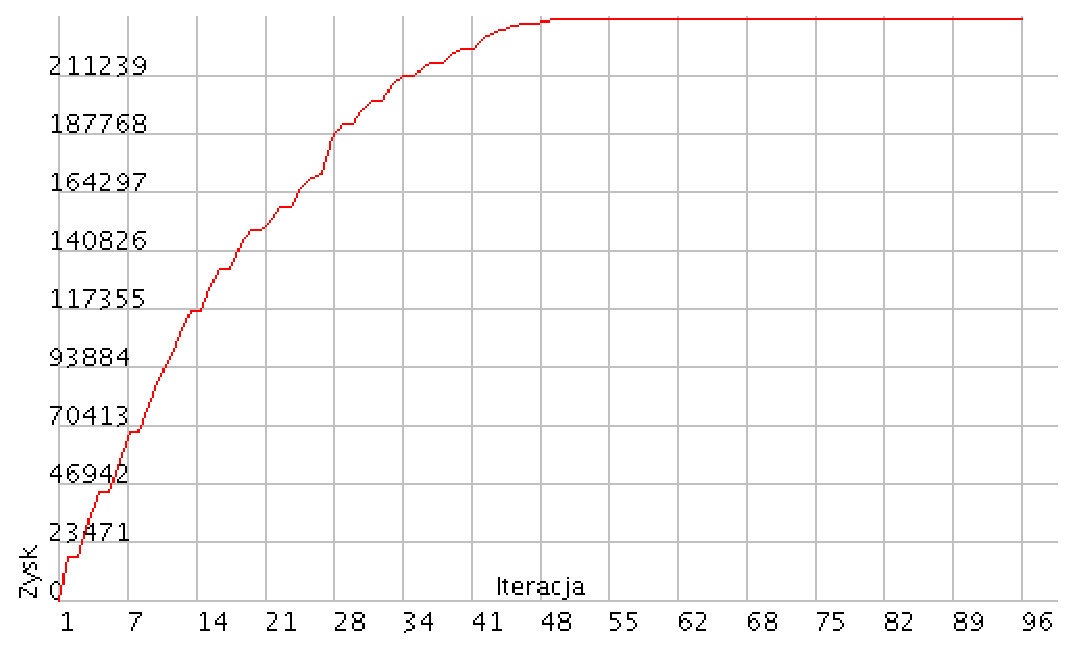
\includegraphics[width=0.45\textwidth]{./img/output/map10_graph.eps}}
  \caption{Mapa map10 : rozwi�zanie oraz wykres funkcji celu}
  \label{fig:map10}
\end{figure}

\begin{figure}
	\begin{tabular}{|r|r|r|}
	\hline
	Nazwa Mapy&Najlepsze rozwi�zanie&czas przetwarzania (ms)\\
	\hline
	map01&6800&24\\
	map02&15500&77\\
	map03&43400&234\\
	map04&40800&668\\
	map05&86100&1043\\
	map06&283400&61841\\
	map07&388900&426915\\
	map08&246200&82253\\
	map09&342500&55507\\
	map10&234700&25765\\
	\hline
	\end{tabular}
\caption{Podsumowanie wynik�w}
\label{tab:summarize}
\end{figure}
\section{Wnioski}
Z przeprowadzonych test�w wynika, �e program nasz dzia�a poprawnie i proponowane rozwi�zania wygl�daj� poprawnie i zgodnie z oczekiwaniami. Potwierdzi�y si� r�wnie� nasze przypuszczenia o wydajno�ci algorytmu, co pozwala na rozwi�zywanie bardziej skomplikowanych map w rozs�dnym czasie.\\
Metoda Tabu Search okaza�a si� skuteczna i szybka. Prawdopodobnie gdyby�my chcieli wykonywa� obliczenia algorytmem �cis�ym trwa�y by one bardzo d�ugo. Dzi�ki zastosowaniu algorytmu przybli�onego czas ten jest bardzo przyzwoity, dla ma�ych map wr�cz pomijalny (rz�du dziesi�tek milisenkund). Pozwala to s�dzi�, �e zaproponowany przez nas model sprawdza si� i mo�e znale�� bardziej praktyczne zastosowanie.\\
Dodatkowo mo�na nieco zmieni� rozumowanie i rozpatrywa� budynki jako np wioski, co pozwoli na takie rozlokowanie anten, aby przykry� nimi jak najwi�ksz� ilo�� wsi (tak mo�na popatrzy� np. na mapk� "map10").


\clearpage
\addcontentsline{toc}{section}{Literatura}
\begin{thebibliography}{99}
\bibitem{bib:onelecture} Wyk�ad z przedmiotu: Badania Operacyjne - K. Wala
\bibitem{bib:oneurl} http://www.ifi.uio.no/infheur/Bakgrunn/Intro\_to\_TS\_Gendreau.htm
\end{thebibliography}

\end{document}
